\chapter{Codifica}

Questo capitolo tratta gli aspetti più interessanti della codifica dell'applicazione moviORDER. In particolare, il capitolo è stato diviso in sezioni che trattano la codifica di:
\begin{enumerate}
	\item \textbf{servizio web};
	\item \textbf{logica applicativa};
	\item \textbf{interfaccia grafica}.
\end{enumerate}

\section{Servizio web}

Per lo sviluppo del servizio web che permette all'applicazione di accedere al database presente sul server cloud di \visione{} si è utilizzato il linguaggio Java e, nello specifico, gli oggetti servlet. Per permettere agli oggetti servlet di interagire con il database si sono dovuti utilizzare i driver JDBC per SQL Server, in quanto moviORDER è basata su tale database. 

\subsection{Servlet}

In questa sezione viene presentato l'utilizzo degli oggetti servlet nella realizzazione del servizio web. Le classi che implementano gli oggetti servlet appartengono al package \textit{servlet}.

\subsubsection{Struttura di un oggetto servlet}

Un oggetto servlet è una classe Java che eredita dalla classe \textit{HttpServlet}, appartenente al package \textit{javax.servlet.http}. \textit{HttpServlet} è una classe astratta che può essere estesa per creare un servlet HTTP utilizzabile per un sito web. Nel progetto realizzato, il servlet è stato utilizzato per acquisire richieste HTTP POST, per elaborarle interrogando il database sul server cloud di \visione{}, e per rispondere ad esse tramite una stringa in formato JSON. Ogni servlet del servizio web implementa il metodo \textit{protected void doPost(HttpServletRequest req, HttpServletResponse resp)}. Tale metodo viene chiamato dal server per permettere all'oggetto servlet di acquisire una richiesta POST da parte di un client. Nel caso del progetto, il client è la logica applicativa dell'applicazione moviORDER e il server è Apache Tomcat.

\textit{HttpServletRequest} è la classe Java che rappresenta le richieste HTTP che possono essere inviate all'oggetto servlet. Tramite opportuni metodi è possibile accedere alle informazioni contenute nella specifica richiesta. Tramite il metodo \textit{String getParameter(String name)} è possibile, data una stringa rappresentante un parametro della richiesta HTTP, ottenere una stringa contenente il valore associato a tale parametro, oppure il valore \textit{null} se il parametro non esiste.

\textit{HttpServletResponse} è la classe Java che rappresenta la risposta dell'oggetto servlet alla richiesta del client. Tramite opportuni metodi è possibile configurare la risposta:
\begin{itemize}
	\item \textit{void setContentType(String type)}: permette di impostare la tipologia di contenuto della risposta. Nel progetto la risposta è una stringa in formato JSON, quindi è stato impostato il content type \textit{application/json};
	\item \textit{PrintWriter getWriter()}: restituisce un oggetto \textit{PrintWriter} che può essere utilizzato per inviare caratteri di testo al client. Nel progetto, l'oggetto \textit{PrintWriter} è stato utilizzato per inviare la stringa di risposta in formato JSON.
\end{itemize}

Viene di seguito fornita, a titolo d'esempio, l'implementazione del metodo \textit{doPost()} del servlet del servizio web che si occupa di controllare che le credenziali inserite dall'utente in fase di login siano corrette. Nella prossima sezione viene fornito un esempio di come la logica applicativa di moviORDER effettua una richiesta a tale servlet e di come utilizza la risposta per modificare lo stato dell'applicazione. Nell'esempio, la classe \textit{DatabaseConnection} fornisce un'interfaccia per l'interrogazione di un database SQL Server. Una spiegazione di tale classe è presente in sezione \ref{dbconnect}.

\begin{figure}[!h] 
    \centering 
    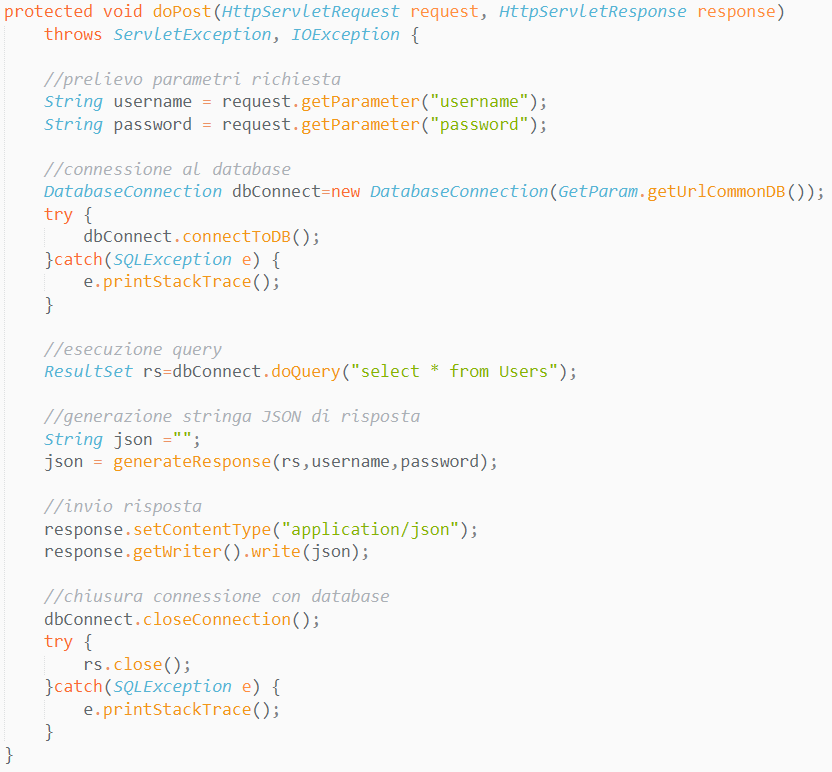
\includegraphics[height=10cm,width=\columnwidth]{codice/servlet} 
    \caption{Metodo \textit{doPost()} del servlet che gestisce l'autenticazione}
\end{figure}

\subsubsection{Interrogazione del servizio web}

Nel momento in cui viene implementato un servlet concreto, eclipse gli associa un end-point in automatico. Tramite l'end-point è possibile raggiungere il servlet sul server per effettuare richieste HTTP. L'end-point associato da eclipse è della forma \textit{/NomeClasseServlet} e puo' essere cambiato dalle impostazioni dell'IDE. Per rendere possibile il raggiungimento del servizio web da parte della logica applicativa di moviORDER, è necessario che venga effettuato il deploy del servizio su Apache Tomcat e che quest'ultimo venga fatto girare sul server cloud di \visione{}. Una volta che il servizio web è raggiungibile tramite la rete, è possibile iniziare ad effettuare richieste HTTP. In moviORDER, la struttura dell'URL di una richiesta HTTP è la seguente: \textit{http://indirizzo:porta/moviORDER/NomeServlet}, dove:
\begin{itemize}
	\item \textit{indirizzo}: è l'indirizzo del server dove il servizio web viene fatto girare:
	\item \textit{porta}: è la porta del server dove il servizio web viene fatto girare;
	\item \textit{NomeServlet}: è l'end-point (servlet) a cui si vuole inviare la richiesta HTTP.
\end{itemize}

MoviORDER effettua richieste HTTP tramite l'utilizzo di AJAX (Asynchronous JavaScript And XML). È importante far notare che AJAX non è un linguaggio di programmazione, bensì una tecnica per accedere ad un server web da una pagina web. Tramite AJAX è possibile leggere dati da un server web dopo che una pagina è stata caricata, aggiornare una pagina web senza il bisogno di dover ricaricare la stessa e inviare dati ad un server web in maniera del tutto trasparente all'utente. 

Nel progetto, AJAX è stato implementato mediante JavaScript con l'utilizzo dell'oggetto \textit{XMLHttpRequest}. Tale oggetto è supportato da tutti i browser moderni e può essere utilizzato per scambiare dati con un server web in maniera trasparente, ovvero senza il bisogno di dover ricaricare la pagina web per cambiarne lo stato. La sintassi per la creazione di un oggetto \textit{XMLHttpRequest} è la seguente:
\textit{var xhttp = new XMLHttpRequest();}. 

Per l'invio di richieste HTTP al servizio web si utilizzano i metodi \textit{open()} e \textit{send()} di \textit{XMLHttpRequest}. In particolare, il metodo \textit{open()} permette di specificare la tipologia di richiesta tramite il passaggio di tre parametri:
	\begin{itemize}
		\item \textbf{metodo}: specifica il metodo utilizzato per inviare la richiesta HTTP: GET o POST;
		\item \textbf{url}: specifica l'indirizzo del server a cui inviare la richiesta HTTP. Nel caso del progetto l'indirizzo comprende l'end-point presso il quale la richiesta deve essere gestita;
		\item \textbf{asincrona/sincrona}: specifica se la richiesta è asincrona (true) o sincrona (false).
	\end{itemize}
Il metodo \textit{send(string)} permette invece l'invio di una richiesta HTTP al servizio web. Esso richiede il passaggio di una stringa contenente i parametri da inviare al server. Poiché alcuni parametri possono contenere caratteri accentati, è stato necessario utilizzare il metodo \textit{setRequestHeader()} per specificare la codifica dei caratteri, aggiungendo header HTTP alla richiesta. Facendo questo, è stato possibile evitare errori di lettura/scrittura di stringhe con caratteri accentati sul database di moviORDER. 

È importante far notare che tutte le richieste HTTP inviate da moviORDER al servizio web sono asincrone, questo perché:
\begin{itemize}
	\item il codice sincrono non è raccomandato poiché JavaScript stopperebbe l'esecuzione fino all'arrivo di una risposta da parte del server. Se il server è occupato o lento, l'applicazione potrebbe aspettare per un tempo prolungato;
	\item le richieste AJAX di tipo sincrono saranno rimosse dallo standard web nei prossimi anni. Scegliendo di utilizzare solamente richieste asincrone si permette a moviORDER di essere robusta a questo cambiamento futuro.
\end{itemize} 

Per la gestione della risposta ricevuta dal server si sono utilizzate le seguenti proprietà dell'oggetto \textit{XMLHttpRequest}:
\begin{itemize}
	\item \textit{readyState}: contiene lo stato dell'oggetto. In particolare, per lo scopo del progetto, è interessante sapere che il valore 4 corrisponde ad una richiesta la cui risposta è pronta;
	\item  \textit{status}: contiene il messaggio sullo stato della richiesta. In particolare, per lo scopo del progetto, è interessante sapere che il valore 200 corrisponde al messaggio OK, che nello standard web rappresenta una richiesta HTTP andata a buon fine;
	\item \textit{onreadystatechange}: definisce una funzione che deve essere eseguita quando la proprietà \textit{readyState} cambia valore;
	\item \textit{responseText}: incapsula la stringa di risposta ricevuta dal servizio web. 
\end{itemize} 
Poiché la risposta ricevuta dal servizio web è una stringa in formato JSON, per effettuare il parsing di tale stringa è stato necessario convertirla in un oggetto JavaScript, tramite l'utilizzo del metodo \textit{JSON.parse()}.

Viene di seguito fornito, a titolo d'esempio, il codice JavaScript della logica applicativa di moviORDER che effettua una chiamata HTTP all'end-point (servlet) che si occupa di gestire l'autenticazione. Il codice si occupa anche di gestire la risposta ricevuta dal servizio web. La funzione \textit{tryLogin()} viene eseguita nel momento in cui l'utente preme sul pulsante di login presente nella schermata di login dell'applicazione.

\newpage

\begin{figure}[!h] 
    \centering 
    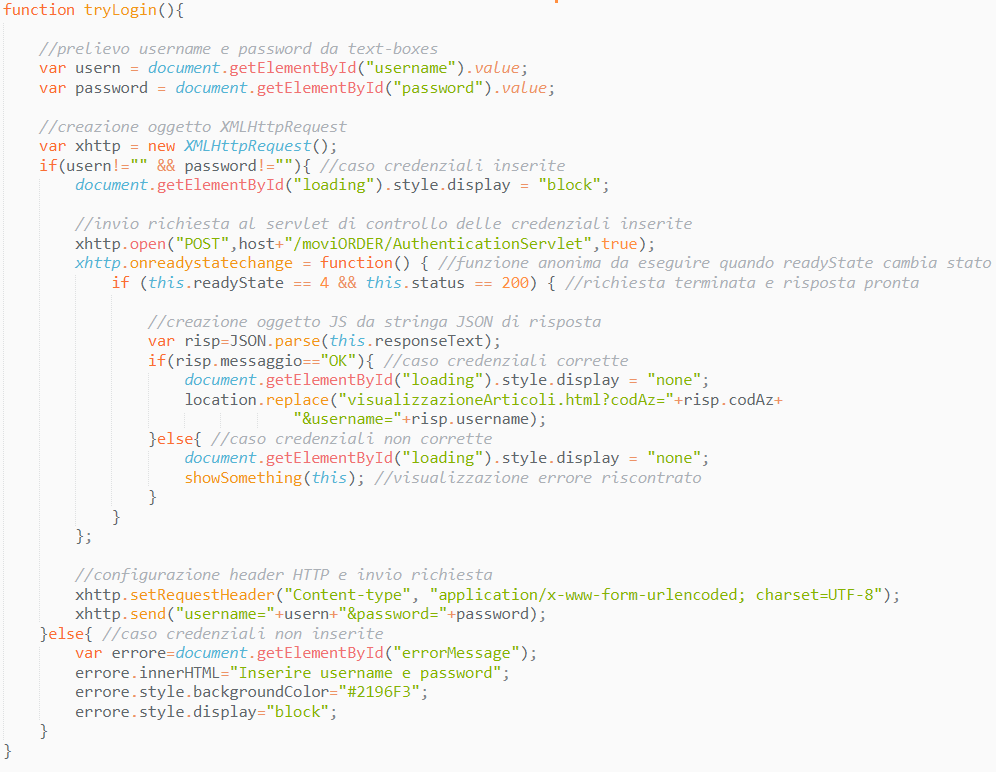
\includegraphics[width=\columnwidth]{codice/ajax} 
    \caption{Esempio di invio di una richiesta HTTP tramite AJAX}
\end{figure}

\subsubsection{API del servizio web} \label{api}

In questa sezione viene presentata la API del servizio web di moviORDER. In particolare, per ogni end-point (servlet) vengono specificati:
\begin{itemize}
	\item \textbf{indirizzo}: indirizzo tramite il quale è possibile raggiungere l'end-point;
	\item \textbf{input}: costituito dai parametri inviati al servizio web tramite una richiesta HTTP;
	\item \textbf{output}: costituito da una stringa in formato JSON che presenta struttura diversa a seconda dell'end-point che gestisce la richiesta;
	\item \textbf{descrizione}.
\end{itemize}

\myparagraph{Servizio di autenticazione}

\begin{itemize}
	\item \textbf{Indirizzo}: /AuthenticationServlet;
	\item \textbf{Input}: il servlet richiede i seguenti parametri:
		\begin{itemize}
			\item \textit{username}: è la username inserita dall'utente in fase di login;
			\item \textit{password}: è la password inserita dall'utente in fase di login.
		\end{itemize}
	\item \textbf{Output}: le possibili risposte del servlet sono le seguenti:
		\begin{itemize}
			\item codice azienda e username dell'utente nel caso in cui username e password passati come parametro corrispondono ad un utente presente in database;
			\item un messaggio d'errore nel caso in cui le credenziali sono scorrette o l'utente è stato bloccato. 
		\end{itemize}
		\item \textbf{Descrizione}: questo servlet rappresenta il servizio di autenticazione di moviORDER. Ricevuti i parametri, il servlet cerca la username dell'utente nel database e, nel caso in cui questa fosse presente, procede nel cercare la password corrispondente. Nel caso in cui username e password passati siano quelli corretti, il servlet restituisce una stringa JSON contenente il codice azienda e la username dell'utente che ha cercando di loggarsi. Nel caso in cui le credenziali non siano corrette, oppure l'utente è stato bloccato, viene restituito un messaggio d'errore.
\end{itemize}

\myparagraph{Servizio di verifica di connessione con il database}

\begin{itemize}
	\item \textbf{Indirizzo}: /CheckConnectionURL;
	\item \textbf{Input}: il servlet richiede i seguenti parametri:
		\begin{itemize}
			\item \textit{codice azienda}: è il codice azienda dell'azienda cliente di \visione{} della quale si vuole verificare la presenza del database.
		\end{itemize}
	\item \textbf{Output}: le possibili risposte del servlet sono le seguenti:
		\begin{itemize}
			\item un messaggio positivo nel caso in cui il database dell'azienda corrispondente al codice inserito è raggiungibile;
			\item un messaggio negativo nel caso in cui il database dell'azienda corrispondente al codice inserito non è raggiungibile.
		\end{itemize}
	\item \textbf{Descrizione}: questo servlet si occupa di controllare se un database aziendale è raggiungibile provando ad effettuare una query su tale database. Risponde positivamente nel caso in cui il database dell'azienda corrispondente al codice inserito è raggiungibile (query con un ritorno), mentre risponde negativamente nel caso in cui il database non è raggiungibile (query che ha sollevato un eccezione).
\end{itemize}

\myparagraph{Servizio di rimozione articoli dal carrello}

\begin{itemize}
	\item \textbf{Indirizzo}: /DeleteSelectedItems;
	\item \textbf{Input}: il servlet richiede i seguenti parametri:
		\begin{itemize}
			\item \textit{lista di codici articolo}: è una lista dei codici articolo degli articoli che devono essere eliminati;
			\item \textit{username}: è la username dell'utente che ha richiesto l'eliminazione degli articoli;
			\item \textit{path}: è la stringa di connessione al database aziendale dell'utente autenticato.
		\end{itemize}
	\item \textbf{Output}: le possibili risposte del servlet sono le seguenti:
		\begin{itemize}
			\item un messaggio positivo nel caso in cui la cancellazione è andata a buon fine;
			\item un messaggio negativo nel caso in cui la cancellazione non è andata a buon fine.
		\end{itemize}
	\item \textbf{Descrizione}: questo servlet si occupa di eliminare dal database aziendale dell'utente autenticato gli articoli che quest'ultimo ha richiesto di rimuovere dal carrello. Risponde positivamente nel caso in cui gli articoli sono stati rimossi correttamente dal database, mentre risponde negativamente nel caso in cui gli articoli non sono stati rimossi dal database.
\end{itemize}

\myparagraph{Servizio di ricerca di un codice a barre}

\begin{itemize}
	\item \textbf{Indirizzo}: /FindArticleBarCode;
	\item \textbf{Input}: il servlet richiede i seguenti parametri:
		\begin{itemize}
			\item \textit{codice a barre}: è il codice a barre di un articolo del quale si vuole conoscere il codice articolo;
			\item \textit{path}: è la stringa di connessione al database aziendale dell'utente autenticato.
		\end{itemize}
	\item \textbf{Output}: le possibili risposte del servlet sono le seguenti:
		\begin{itemize}
			\item codice articolo corrispondente al barcode passato come parametro nel caso in cui il barcode corrisponde a quello di un articolo venduto dall'azienda;
			\item un messaggio negativo nel caso in cui il barcode passato come parametro non corrisponde ad un articolo venduto dall'azienda.
		\end{itemize}
	\item \textbf{Descrizione}: questo servlet si occupa di fornire il codice articolo dell'articolo corrispondente al codice a barre ricevuto come parametro, effettuando la ricerca del barcode all'interno del database. Nel caso in cui il codice a barre è presente all'interno del database viene restituito il codice articolo corrispondente, mentre nel caso in cui non è presente viene restituito un messaggio negativo.
\end{itemize}

\myparagraph{Servizio di ricerca di un codice articolo}

\begin{itemize}
	\item \textbf{Indirizzo}: /FindArticleCode;
	\item \textbf{Input}: il servlet richiede i seguenti parametri:
		\begin{itemize}
			\item \textit{codice articolo}: è il codice articolo o il barcode di un articolo del quale si vuole verificare la presenza in database;
		\end{itemize}
	\item \textbf{Output}: le possibili risposte del servlet sono le seguenti:
		\begin{itemize}
			\item codice articolo nel caso in cui l'articolo è presente in database;
			\item un messaggio negativo nel caso in cui l'articolo non è presente in database.
		\end{itemize}
	\item \textbf{Descrizione}: questo servlet si occupa di fornire il codice articolo dell'articolo corrispondente al codice articolo o al barcode ricevuto come parametro, effettuando la ricerca del codice articolo o del barcode all'interno del database. Nel caso in cui il codice articolo o il barcode passato come parametro corrisponde ad un articolo presente in database viene restituito il codice articolo, mentre nel caso in cui non corrisponde ad un articolo presente in database viene restituito un messaggio negativo.
\end{itemize}

\myparagraph{Servizio di prelievo informazioni di un articolo}

\begin{itemize}
	\item \textbf{Indirizzo}: /GetArticleDescNote;
	\item \textbf{Input}: il servlet richiede i seguenti parametri:
		\begin{itemize}
			\item \textit{codice azienda}: è il codice azienda della quale l'utente autenticato è cliente;
			\item \textit{codice articolo}: è il codice articolo dell'articolo del quale si vogliono ottenere informazioni.
		\end{itemize}
	\item \textbf{Output}: questo servlet può produrre un solo output poiché l'applicazione è stata implementata in modo che non ci siano casi negativi:
		\begin{itemize}
			\item descrizione, note, quantità minima ordinabile e step di incremento quantità per l'articolo corrispondente al codice articolo passato come parametro.
		\end{itemize}
	\item \textbf{Descrizione}: questo servlet si occupa di fornire informazioni sull'articolo corrispondente al codice articolo passato come parametro. 
\end{itemize}

\myparagraph{Servizio di prelievo degli articoli in carrello}

\begin{itemize}
	\item \textbf{Indirizzo}: /GetArticlesByUsername;
	\item \textbf{Input}: il servlet richiede i seguenti parametri:
		\begin{itemize}
			\item \textit{codice azienda}: è il codice azienda della quale l'utente autenticato è cliente;
			\item \textit{username}: è il nome utente dell'utente autenticato.
		\end{itemize}
	\item \textbf{Output}: le possibili risposte del servlet sono le seguenti:
		\begin{itemize}
			\item array degli articoli nel carrello dell'utente autenticato, dove per ogni articolo vengono restituiti la quantità ordinata, il codice articolo e la descrizione dell'articolo;
			\item array vuoto nel caso in cui l'utente autenticato non presenta articoli in carrello.
		\end{itemize}
	\item \textbf{Descrizione}: questo servlet si occupa di fornire la lista degli articoli in carrello per l'utente la quale username è stata passata come parametro. Nel caso in cui l'utente presenta articoli in carrello viene restituita la lista degli articoli in carrello, mentre nel caso in cui non presenta articoli in carrello viene restituita una lista vuota.
\end{itemize}

\myparagraph{Servizio di prelievo di informazioni di un utente}

\begin{itemize}
	\item \textbf{Indirizzo}: /GetNameByUsername;
	\item \textbf{Input}: il servlet richiede i seguenti parametri:
		\begin{itemize}
			\item \textit{path}: è la stringa di connessione al database aziendale dell'utente autenticato;
			\item \textit{username}: è il nome utente dell'utente autenticato.
		\end{itemize}
	\item \textbf{Output}: questo servlet può produrre un solo output poiché l'applicazione è stata implementata in modo che non ci siano casi negativi:
		\begin{itemize}
			\item nome e ragione sociale dell'utente autenticato e codice documento e descrizione del documento da generare nel caso in cui l'utente invii un ordine.
		\end{itemize}
	\item \textbf{Descrizione}: questo servlet si occupa di fornire informazioni sull'utente la cui username è stata passata come parametro.
\end{itemize}

\myparagraph{Servizio di prelievo informazioni di un articolo in carrello}

\begin{itemize}
	\item \textbf{Indirizzo}: /GetTmpArticleData;
	\item \textbf{Input}: il servlet richiede i seguenti parametri:
		\begin{itemize}
			\item \textit{path}: è la stringa di connessione al database aziendale dell'utente autenticato;
			\item \textit{codice articolo}: è il codice articolo dell'articolo del quale si vogliono ottenere informazioni;
			\item \textit{username}: è il nome utente dell'utente autenticato.
		\end{itemize}
	\item \textbf{Output}: questo servlet può produrre un solo output poiché l'applicazione è stata implementata in modo che non ci siano casi negativi:
		\begin{itemize}
			\item quantità e note dell'articolo nel carrello dell'utente autenticato corrispondente al codice articolo passato come parametro.
		\end{itemize}
	\item \textbf{Descrizione}: questo servlet si occupa di fornire informazioni riguardati uno specifico articolo nel carrello dell'utente la quale username è stata passata come parametro.
\end{itemize}

\myparagraph{Servizio di inserimento/modifica articolo}

\begin{itemize}
	\item \textbf{Indirizzo}: /InsertUpdateArticle;
	\item \textbf{Input}: il servlet richiede i seguenti parametri:
		\begin{itemize}
			\item \textit{path}: è la stringa di connessione al database aziendale dell'utente autenticato;
			\item \textit{query}: è una stringa contenente la query di inserimento/modifica di un articolo.
		\end{itemize}
	\item \textbf{Output}: le possibili risposte del servlet sono le seguenti:
		\begin{itemize}
			\item un messaggio positivo nel caso in cui la query di inserimento/modifica articolo è andata a buon fine;
			\item un messaggio negativo nel caso in cui la query di inserimento/modifica articolo non è andata a buon fine.
		\end{itemize}
	\item \textbf{Descrizione}: questo servlet si occupa di inserire o modificare un articolo nel carrello dell'utente autenticato. L'inserimento e la modifica avvengono mediante l'utilizzo dello stesso servlet poiché la query da eseguire sul database, che può essere di tipo INSERT o UPDATE, viene passata come parametro. Nel caso in cui la query viene eseguita in modo corretto sul database viene restituito un messaggio positivo, mentre nel caso in cui non viene eseguita viene restituito un messaggio negativo.
\end{itemize}

\myparagraph{Servizio di invio di un ordine}

\begin{itemize}
	\item \textbf{Indirizzo}: /SendOrder;
	\item \textbf{Input}: il servlet richiede i seguenti parametri:
		\begin{itemize}
			\item path: è la stringa di connessione al database aziendale dell'utente autenticato;
			\item codici articolo: è la lista dei codici degli articoli che l'utente autenticato ha ordinato;
			\item username: è il nome utente dell'utente autenticato;
			\item ragione sociale: è la ragione sociale dell'utente autenticato;
			\item nome: è il nome dell'utente autenticato;
			\item codice documento: è il codice del documento che deve essere generato con l'ordine;
			\item data: è la data d'invio dell'ordine;
			\item note: sono le note inserite dall'utente in fase di invio dell'ordine;
			\item codice azienda: è il codice azienda della quale l'utente autenticato è cliente.
		\end{itemize}
	\item \textbf{Output}: le possibili risposte del servlet sono le seguenti:
		\begin{itemize}
			\item un messaggio positivo nel caso in cui l'ordine è stato inviato con successo;
			\item un messaggio negativo nel caso in cui l'ordine non è stato inviato con successo.
		\end{itemize}
	\item \textbf{Descrizione}: questo servlet si occupa di registrare sul database un ordine contenente gli articoli passati come parametro. Il resto dei parametri passati viene utilizzato per inviare una mail di conferma all'utente autenticato e all'azienda presso cui l'utente è cliente. Nel caso in cui la registrazione dell'ordine sul database avvenga correttamente viene restituito un messaggio positivo, mentre nel caso in cui non avvenga correttamente viene restituito un messaggio negativo.
\end{itemize}

\subsection{JDBC}

In questa sezione viene presentato l'utilizzo della Java Database Connectivity API nella realizzazione del servizio web.

\subsubsection{Driver JDBC}

Un driver JDBC è una componente software che permette ad un'applicazione Java di interagire con un database. Per supportare la connessione a singoli database, JDBC (Java Database Connectivity API) richiede i driver per ogni database. Il driver permette la connessione con il database e implementa il protocollo di trasferimento di query e risultati tra il client e il database. Poiché per l'implementazione del database è stato utilizzato SQL Server si sono dovuti utilizzare i driver JDBC per tale database.

\subsubsection{Classe DatabaseConnection} \label{dbconnect}

Per lo sviluppo del servizio web è stata realizzata la classe \textit{DatabaseConnection} appartenente al package \textit{dbConnection}. Tale classe fornisce un'interfaccia utilizzabile per la gestione dell'interazione con un database di tipo SQL Server. In questa sezione vengono presentati i metodi che costituiscono tale interfaccia.

\myparagraph{Costruttori}

La classe presenta due metodi costruttori:
\begin{itemize}
	\item \textit{public DatabaseConnection(String u, String user, String psw, String db)}: costruisce un oggetto \textit{DatabaseConnection} a partire dall'URL del server in cui è presente il database, la username e la password di accesso al database, e il nome del database al quale si desidera connettesi;
	\item \textit{public DatabaseConnection(String dbConnectionString)}: costruisce un oggetto \textit{DatabaseConnection} a partire dalla stringa di connessione ad uno specifico database.
\end{itemize}
Il formato della stringa di connessione ad un database è il seguente: \textit{indirizzoServer;databaseName=nomeDb;user=u;password=psw}, dove:
\begin{itemize}
	\item \textit{indirizzoServer}: è l'indirizzo IP pubblico del server contenente il database al quale si desidera connettersi. Nel caso del progetto potrebbe essere l'indirizzo del server di un'azienda esterna che desidera utilizzare il proprio database per l'interazione;
	\item \textit{nomeDb}: è il nome del database al quale si desidera connettersi;
	\item \textit{u}: è il nome utente per l'accesso al database;
	\item \textit{psw}: è la password per l'accesso al database.
\end{itemize}
Viene di seguito presentato, a titolo d'esempio, il codice Java che implementa il metodo \textit{public DatabaseConnection(String dbConnectionString)}. Il metodo si occupa di splittare la stringa di connessione passata come parametro per ottenere i dati utili alla costruzione dell'oggetto \textit{DatabaseConnection}.

\begin{figure}[!h] 
    \centering 
    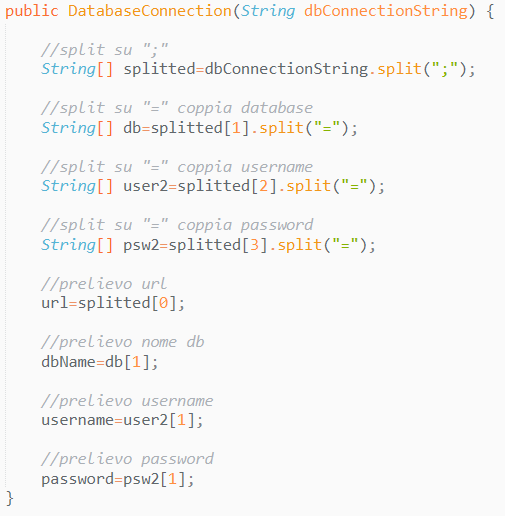
\includegraphics[height=8cm,width=0.8\columnwidth]{codice/databaseCostruttore} 
    \caption{Metodo costruttore della classe \textit{DatabaseConnection}}
\end{figure}

\myparagraph{Metodo \textit{connectToDb()}}

Tale metodo si occupa di instaurare la connessione con il database desiderato. Per far questo, configura i driver JDBC e costruisce l'URL di connessione al database tramite i dati contenuti nell'oggetto d'invocazione. Il metodo potrebbe sollevare un'eccezione di tipo \textit{ClassNotFoundException} nel caso in cui la classe utilizzata per i driver JDBC sia inesistente o non sia stata importata all'interno del progetto. Viene di seguito fornito, a titolo d'esempio, il codice del metodo \textit{connectToDb()}.

\begin{figure}[!h] 
    \centering 
    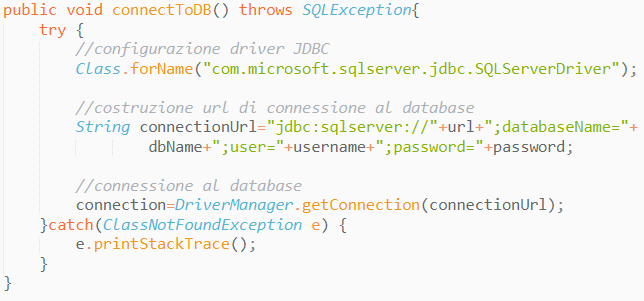
\includegraphics[width=\columnwidth]{codice/connessionedb} 
    \caption{Metodo \textit{connectToDb()} della classe \textit{DatabaseConnection}}
\end{figure}

\myparagraph{Altri metodi}

Sono stati implementati altri metodi di complessità inferiore. Per questo motivo ne viene presentata solamente una breve descrizione:
\begin{itemize}
	\item \textit{doQuery(query)}: questo metodo permette di eseguire una query di tipo SELECT sul database. Restituisce il \textit{ResultSet} contenente il risultato della query;
	\item \textit{doUpdateQuery(query)}: questo metodo permette di eseguire una query di tipo INSERT, UPDATE o DELETE sul database. Restituisce il numero di righe inserite, modificate o cancellate;
	\item \textit{closeConnection()}: questo metodo permette di eseguire il processo di disconnessione dal database.
\end{itemize}

\subsection{Classi utilità}

Per lo sviluppo del servizio web è stato necessario implementare due classi utilità. In questa sezione ne viene presentata brevemente l'implementazione. Tali classi appartengono al package \textit{utility}.

\subsubsection{Classe GetParam}

La classe \textit{GetParam} si occupa di restituisce un campo statico contenente la stringa di connessione al database \textit{CommonDb} dell'applicazione moviORDER. Come detto precedentemente, questo database contiene tutti i dati di autenticazione degli utenti di moviORDER. Poiché tale stringa di connessione viene utilizzata frequentemente all'interno del servizio web, si è deciso di inserirla in un unico punto del servizio, in modo da evitare la modifica di più file nel caso in cui essa cambi.

\subsubsection{Classe MailUtility}

La classe \textit{MailUtility} fornisce un'interfaccia per l'invio di e-mail. È stato necessario implementare tale classe poiché è stato richiesto di inviare una mail di conferma all'utente autenticato e all'azienda presso cui l'utente è cliente nel momento in cui un ordine viene registrato. La classe presenta un costruttore che richiede i parametri per la configurazione di un server SMTP:
\begin{itemize}
	\item \textbf{host}: è l'indirizzo IP dell'host su cui è installato il server SMTP;
	\item \textbf{post}: è il numero di porta dell'host su cui è installato il server SMTP;
	\item \textbf{username}: è il nome utente di accesso al server SMTP;
	\item \textbf{password}: è la password di accesso al server SMTP.
\end{itemize}
Il metodo \textit{sendMail()} si occupa di configurare e inviare una mail all'utente che ha effettuato l'ordine e all'azienda presso cui l'utente è cliente. Per far questo, il metodo richiede:
\begin{itemize}
	\item indirizzo e-mail dell'utente;
	\item indirizzo e-mail dell'azienda;
	\item indirizzo e-mail del mittente;
	\item oggetto della e-mail;
	\item testo della e-mail: è una tabella scritta in codice HTML contenente i dati degli articoli ordinati.
\end{itemize}
Viene di seguito fornito, a titolo d'esempio, il codice Java che implementa il metodo \textit{sendMail()}.

\newpage

\begin{figure}[!h] 
    \centering 
    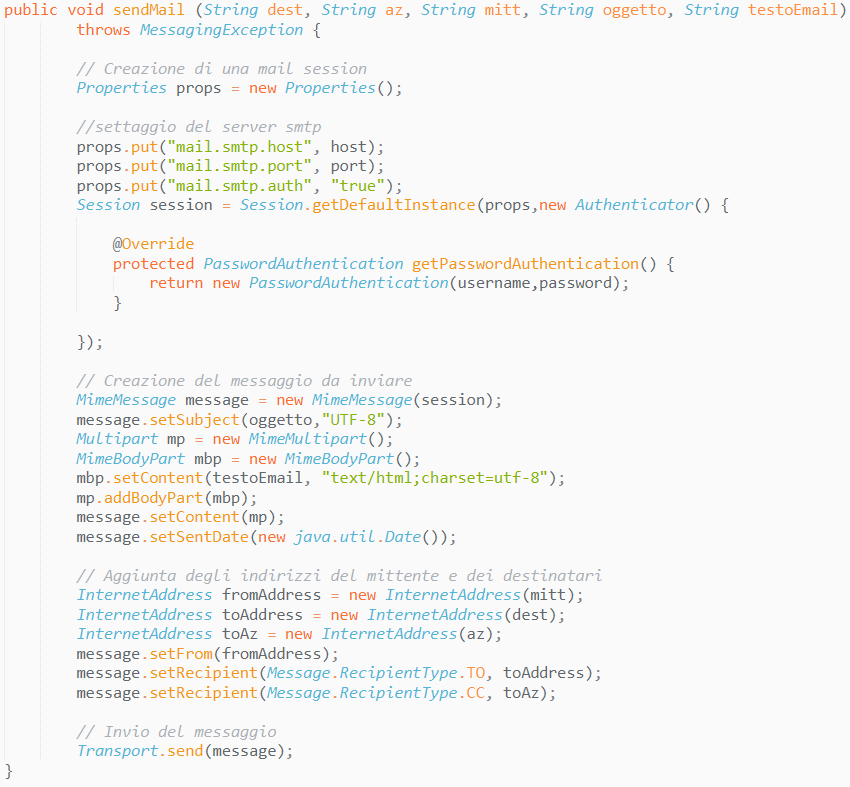
\includegraphics[width=\columnwidth]{codice/mail} 
    \caption{Metodo \textit{sendMail()} della classe \textit{MailUtility}}
\end{figure}

\section{Logica applicativa}

In questa sezione vengono presentati gli aspetti più interessanti riguardanti la codifica della logica applicativa di moviORDER. La sezione si incentra sui meccanismi di integrazione dei plugin PhoneGap con il codice Javascript della logica applicativa.

\subsection{Plugin di PhoneGap}

Un plugin è un pacchetto di codice che permette al visualizzatore web di Cordova, il quale renderizza l'applicazione, di comunicare con la piattaforma nativa sulla quale viene eseguito. I plugin forniscono accesso alle funzionalità del dispositivo e della piattaforma che normalmente non sono disponibili per le applicazioni web-based. Tutte le principali API di Cordova sono implementate tramite plugin. Un aspetto interessante dei plugin è che essi sono composti da un'unica interfaccia JavaScript che astrae le differenti librerie di codice nativo delle piattaforme supportate dal plugin. Quindi, essenzialmente, i plugin nascondono le varie implementazioni di codice nativo dietro un'interfaccia JavaScript comune.

\subsection{Installazione dei plugin}

Tramite PhoneGap CLI, interfaccia a linea di comando precedentemente descritta, è possibile aggiungere i plugin desiderati alla configurazione del progetto PhoneGap. È sufficiente lanciare la CLI dalla cartella principale del progetto ed eseguire il comando \textit{phonegap plugin add nomePlugin}, dove \textit{nomePlugin} è il nome del plugin che si desidera scaricare e installare (es. \textit{cordova-plugin-whitelist}).

\subsection{Premesse all'utilizzo dei plugin}

Per poter utilizzare i plugin di PhoneGap efficacemente è necessario predisporre il codice JavaScript al loro utilizzo. In particolare sono necessari due accorgimenti che vengono di seguito presentati.

\subsubsection{Inclusione di cordova.js}

In ogni file della logica applicativa che utilizza dei plugin PhoneGap deve essere importato il file \textit{cordova.js}. Questo file JavaScript permette il funzionamento dei plugin utilizzati all'interno della logica di moviORDER. Se si cerca di utilizzare un plugin senza aver importato tale file, la console darà il seguente errore: ``Cordova in not available, Make sure to include cordova.js''.

\subsubsection{Evento deviceready}

L'evento \textit{deviceready} è essenziale in ogni applicazione poiché segnala il corretto caricamento delle API di Cordova sul dispositivo. Se l'evento non venisse atteso prima di utilizzare un plugin, si rischierebbe che l'applicazione effettui una chiamata ad una funzione JavaScript di Cordova prima che il corrispondente codice nativo per il dispositivo diventi disponibile. L'evento \textit{deviceready} viene lanciato una volta che Cordova è stato completamente caricato. Quindi nel momento in cui tale evento viene lanciato, è possibile effettuare chiamate alle API di Cordova in completa sicurezza. Per attendere l'evento è sufficiente inserire un listener nel codice JavaScript. Viene di seguito fornito, a scopo illustrativo, un esempio di codice JavaScript che implementa l'attesa di tale evento.

\begin{figure}[!h] 
    \centering 
    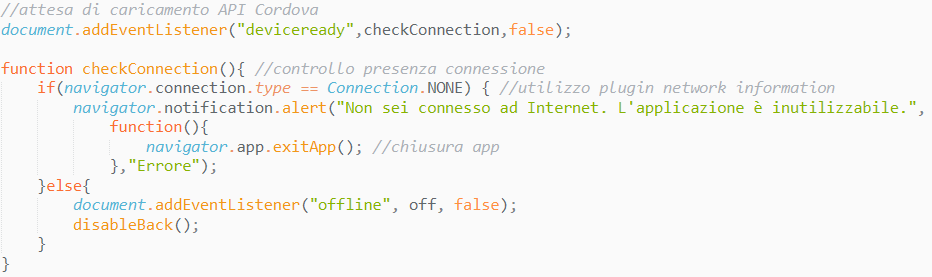
\includegraphics[width=\columnwidth]{codice/deviceready} 
    \caption{Esempio di codice JavaScript che attende l'evento \textit{deviceready}}
\end{figure}

\subsection{Plugin utilizzati}

In questa sezione vengono presentati i plugin PhoneGap utilizzati nella realizzazione della logica applicativa di moviORDER. Per ogni plugin vengono messi in evidenzia vantaggi e svantaggi (se presenti) nell'utilizzo e un esempio di utilizzo.

\subsubsection{Dialogs plugin}

Il plugin \textit{dialogs} fornisce accesso all'interfaccia grafica nativa degli elementi dialog tramite l'utilizzo dell'oggetto \textit{navigator.notification}. Questo plugin è stato utilizzato convertire gli alert box delle pagine web in dialog nativi. Sono stati utilizzati i seguenti metodi:
\begin{itemize}
	\item \textit{alert()}: visualizza un dialog box nativo con un messaggio di allerta preimpostato. Il metodo richiede i seguenti parametri:
	\begin{itemize}
		\item \textit{message}: è il messaggio visualizzato nel dialog;
		\item \textit{callback}: è una funzione anonima di callback da eseguire quando viene premuto il pulsante nel dialog;
		\item \textit{title}: è il titolo del dialog;
		\item \textit{buttonName}: è il testo che viene scritto all'interno del bottone nel dialog.
	\end{itemize}
	\item \textit{confirm()}: visualizza un dialog box nativo per richiedere conferma di un'azione. Il metodo richiede i seguenti parametri:
	\begin{itemize}
		\item \textit{message}: è il messaggio visualizzato nel dialog di conferma;
		\item \textit{callback}: è una funzione anonima di callback da eseguire nel caso in cui il bottone di conferma viene premuto;
		\item \textit{title}: è il titolo del dialog di conferma;
		\item \textit{buttonLabels}: sono le etichette dei vari bottoni presenti nel dialog di conferma. Solitamente sono ``OK'' e ``Annulla''.
	\end{itemize}
\end{itemize}

Senza l'utilizzo di questo plugin non sarebbe stato possibile modificare il titolo e i bottoni del dialog poiché per motivi di sicurezza JavaScript non permette tale modifica. Inoltre la visualizzazione del dialog non sarebbe stata la visualizzazione desiderata, ovvero quella nativa. 

Vengono di seguito forniti, a scopo illustrativo, un esempio di codice JavaScript che non utilizza il plugin e un esempio che lo utilizza. Per ognuno degli esempi viene mostrato uno screenshot dell'output risultante che, nel primo caso sarà un comune alert e nel secondo un dialog nativo.

\begin{figure}[!h] 
    \centering 
    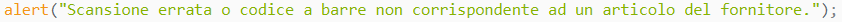
\includegraphics[width=\columnwidth]{codice/alert} 
    \caption{Esempio di codice JavaScript che non utilizza il plugin \textit{dialogs}}
\end{figure}

\newpage

\begin{figure}[!h] 
    \centering 
    \includegraphics[width=0.4\columnwidth]{codice/imgalert} 
    \caption{Esempio di visualizzazione scorretta - alert}
\end{figure}

\begin{figure}[!h] 
    \centering 
    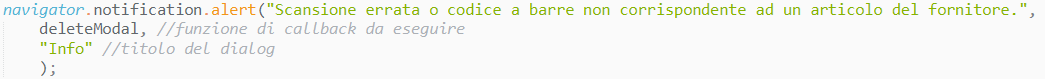
\includegraphics[width=\columnwidth]{codice/dialog} 
    \caption{Esempio di codice JavaScript che utilizza il plugin \textit{dialogs}}
\end{figure}

\begin{figure}[!h] 
    \centering 
    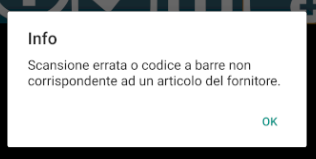
\includegraphics[width=0.4\columnwidth]{codice/imgDialog} 
    \caption{Esempio di visualizzazione corretta - dialog}
\end{figure}

\subsubsection{Network information plugin}

Il plugin \textit{network information} fornisce una moderna implementazione della Network Information API. Essa fornisce informazioni riguardanti la rete cellulare e Wi-Fi del dispositivo e permette di capire se il dispositivo presenta una connessione a Internet. Più precisamente, il plugin fornisce un'interfaccia JavaScript che astrae il codice nativo utilizzato per monitorare la rete del dispositivo. L'oggetto \textit{navigator.connection} permette di acquisire le informazioni appena descritte. È stata utilizzata la proprietà \textit{type} per comprendere in modo veloce lo stato della connessione del dispositivo e la tipologia di connessione attiva. La proprietà può assumere i seguenti valori:
\begin{itemize}
	\item \textit{Connection.UNKNOWN}: tipologia di rete sconosciuta;
	\item \textit{Connection.ETHERNET}: dispositivo connesso alla rete via cavo ethernet;
	\item \textit{Connection.WIFI}: dispositivo connesso ad una rete Wi-Fi;
	\item \textit{Connection.CELL\_2G}: dispositivo connesso ad una rete cellulare di tipo 2G;
	\item \textit{Connection.CELL\_3G}: dispositivo connesso ad una rete cellulare di tipo 3G;
	\item \textit{Connection.CELL\_4G}: dispositivo connesso ad una rete cellulare di tipo 4G;
	\item \textit{Connection.CELL}: dispositivo connesso ad una rete cellulare la cui tipologia non è identificabile;
	\item \textit{Connection.NONE}: dispositivo non connesso alla rete.
\end{itemize}
Un limite di questa proprietà è presente in ambiente iOS, infatti non è possibile identificare nessun tipo di rete cellulare alla quale il dispositivo è connesso. Per questo in ambiente iOS di è dovuta utilizzare la proprietà \textit{onLine} dell'oggetto \textit{navigator}.

All'oggetto \textit{navigator.connection} sono collegate due tipologie di evento:
\begin{itemize}
	\item \textit{offline}: viene lanciato quando un dispositivo precedentemente collegato ad Internet perde la connessione e l'applicazione non è più in grado di accedere alla rete. In particolare, viene lanciato esattamente quando il valore della proprietà \textit{type} diventa \textit{Connection.NONE};
	\item \textit{online}: viene lanciato quando un dispositivo precedentemente scollegato dalla rete riceve la connessione e permette all'applicazione di accedere ad Internet. In particolare, viene lanciato esattamente quando il valore della proprietà \textit{type} cambia da \textit{NONE} ad un altro valore.
\end{itemize}
Il plugin \textit{network information} è stato utilizzato per chiudere l'applicazione nel caso in cui venisse aperta mentre il dispositivo è offline. L'evento \textit{offline} ha permesso inoltre di visualizzare messaggi relativi allo stato della connessione. In particolare, nel caso in cui il dispositivo perdesse la connessione durante l'utilizzo di moviORDER viene visualizzato un messaggio che notifica all'utente che l'applicazione è inutilizzabile.

Vengono di seguito forniti, a scopo illustrativo, un esempio di codice JavaScript che utilizza \textit{network.connection} ed in particolare la proprietà \textit{type} e l'evento \textit{offline}.

\begin{figure}[!h] 
    \centering 
    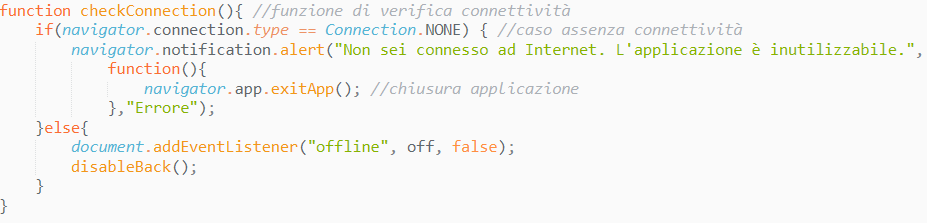
\includegraphics[width=\columnwidth]{codice/type} 
    \caption{Esempio di utilizzo della proprietà \textit{type}}
\end{figure}

\begin{figure}[!h] 
    \centering 
    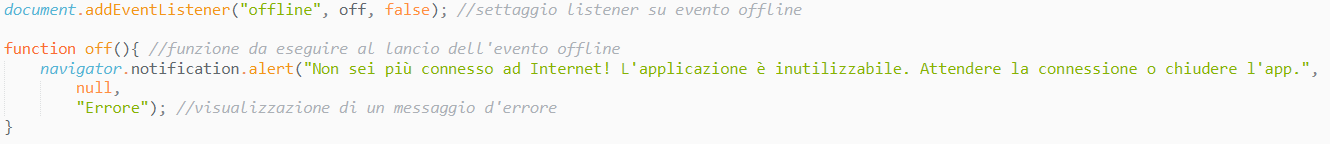
\includegraphics[width=\columnwidth]{codice/offline} 
    \caption{Esempio di utilizzo dell'evento \textit{offline}}
\end{figure}

\subsubsection{Barcode scanner plugin}

Il plugin \textit{barcode scanner} fornisce un'interfaccia JavaScript che astrae il codice nativo che permette di effettuare la scansione di un codice a barre da un qualsiasi dispositivo dotato di fotocamera. Il plugin crea l'oggetto \textit{cordova.plugin.barcodeScanner} che presenta il metodo \textit{scan(success, fail, settings)}. \textit{Success} è la funzione di callback da eseguire quando la scansione del codice a barre va a buon fine. \textit{Fail} è la funzione di callback da eseguire quando la scansione del codice a barre non va a buon fine. \textit{Settings} è una variabile contenente un insieme di settaggi per l'utilizzo del plugin:
\begin{itemize}
	\item \textit{preferFrontCamera}: permette di preferire la fotocamera frontale alla posteriore per la scansione del codice a barre;
	\item \textit{showFlipCameraButton}: permette di visualizzare il bottone per il cambio della fotocamera;
	\item \textit{showTorchButton}: permette di visualizzare il bottone per l'attivazione del flash;
	\item \textit{torchOn}: permette di attivare il flash di default;
	\item \textit{saveHistory}: permette il salvataggio della cronologia dei codici scansionati;
	\item \textit{prompt}: permette di visualizzare un messaggio per aiutare l'utente nell'eseguire la scansione;
	\item \textit{resultDisplayDuration}: permette di visualizzare un testo per un determinato numero di secondi nel caso in cui un codice a barre viene captato;
	\item \textit{formats}: permette di settare la tipologia di codici a barre che devono essere captati;
	\item \textit{orientation}: permette di settare l'orientamento del dispositivo durante la scansione del codice a barre;
	\item \textit{disableAnimations}: permette la disattivazione di ogni tipo di animazione durante la scansione del codice a barre;
	\item \textit{disableSuccessBeep}: permette di disabilitare l'emissione del suono acustico nel caso in cui un codice a barre viene captato.
\end{itemize}
In ambiente iOS è necessario aggiungere una \textit{NSCameraUsageDescription} al file \textit{Info.plist} per poter utilizzare corettamente il plugin. \textit{NSCameraUsageDescription} descrive la ragione per la quale l'applicazione accede alla fotocamera dell'utente. Quando il sistema operativo richiede all'utente di permettere l'accesso, la stringa inserita in tale campo viene visualizzata sul dialog box. Se non viene fornita la descrizione di utilizzo l'applicazione crescerà prima della visualizzazione del dialog. Inoltre, Apple rifiuta le applicazioni che accedono a dati privati senza fornire una descrizione di utilizzo. 

Il plugin ha funzionato perfettamente in ambiente Android ma non si può dire lo stesso per l'ambiente iOS. Nei dispositivi con una fotocamera mediocre le scansioni richiedevano più tempo del previsto, alcune volte anche minuti. Per risolvere il problema si è dovuto modificare il codice nativo per la piattaforma iOS. Il problema veniva riscontrato perché il codice differenziava il processo di scansione a seconda della qualità rilevata della fotocamera del dispositivo. Per telefoni con fotocamera mediocre veniva fatta una valutazione troppo ottimistica e per questo si è dovuto modificare il codice in modo da unificare il processo di scansione. Dopo vari test si è potuto osservare che la soluzione migliore era l'utilizzo del processo di scansione con fotocamera di qualità media. Viene di seguito fornito, a scopo illustrativo, il codice Objective-C++ che si occupa di settare il processo di scansione.

\begin{figure}[!h] 
    \centering 
    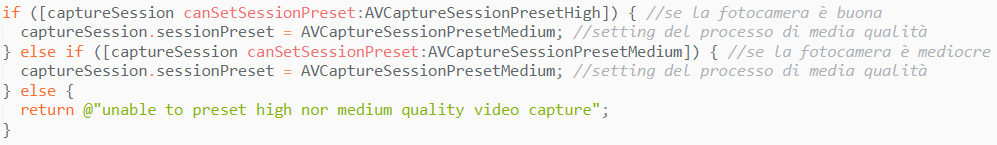
\includegraphics[width=\columnwidth]{codice/scan} 
    \caption{Codice Objective-C++ per il settaggio del processo di scansione}
\end{figure}

Viene di seguito fornito, a scopo illustrativo, il codice JavaScript della logica di moviORDER che utilizza il plugin \textit{barcode scanner}.
\\
\begin{figure}[!h] 
    \centering 
    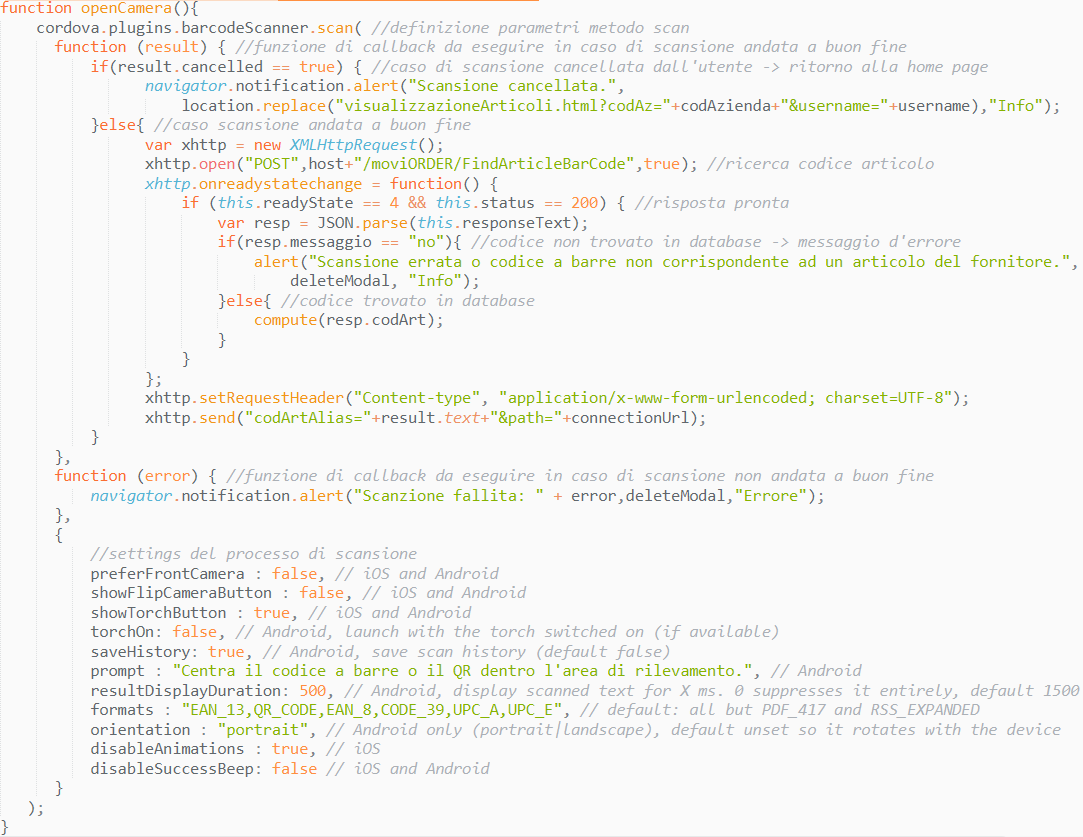
\includegraphics[width=\columnwidth]{codice/scan2} 
    \caption{Codice JavaScript che utilizza il plugin \textit{barcode scanner}}
\end{figure}

\newpage

\section{Interfaccia grafica}

In questa sezione vengono presentati gli aspetti più interessanti della codifica dell'interfaccia grafica di moviORDER. In particolare, vengono presentate le possibili interazioni dell'utente con le interfacce.

\subsection{Schermata di login}

\begin{figure}[!h] 
    \centering 
    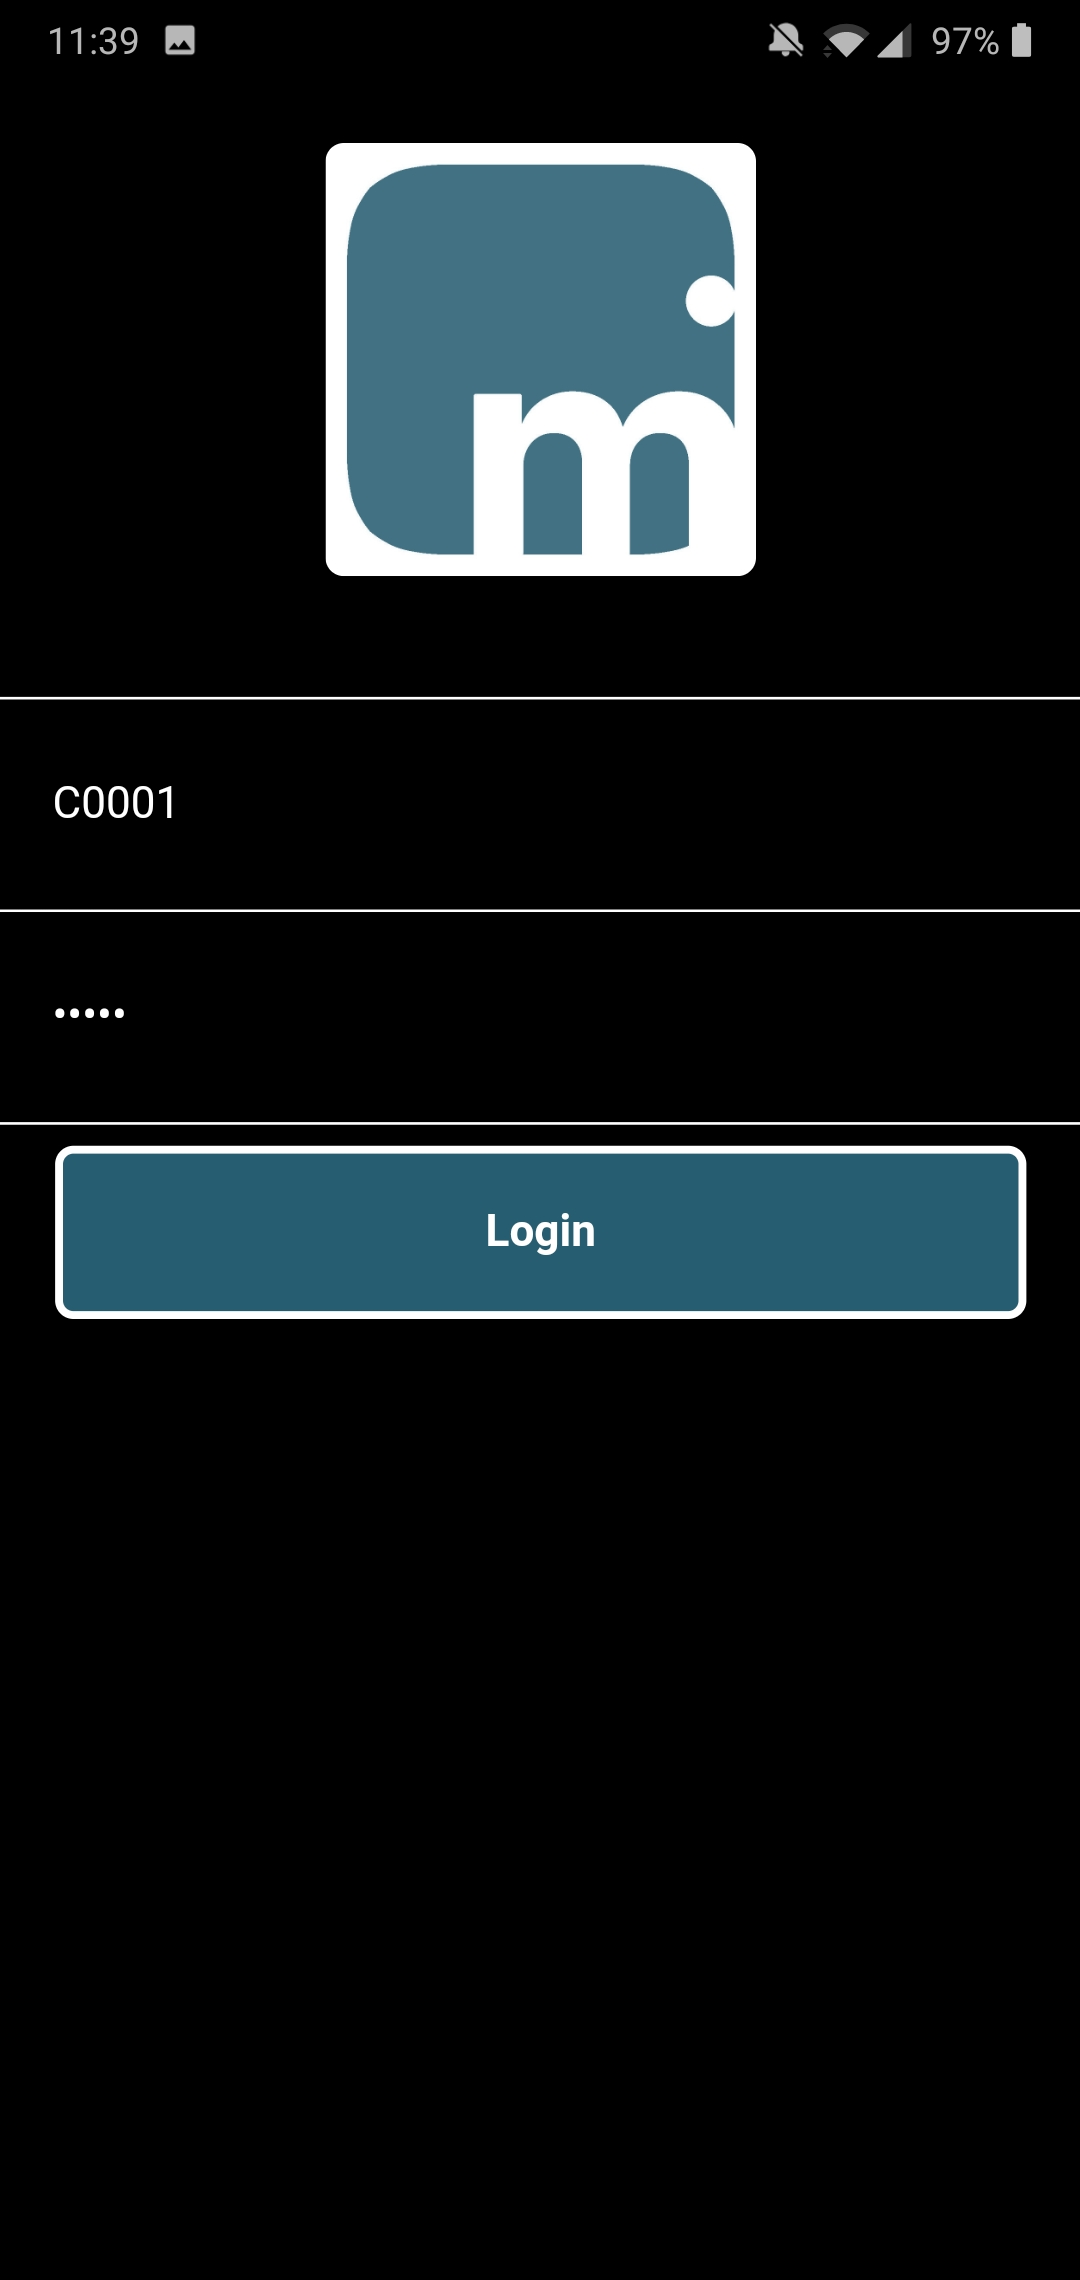
\includegraphics[width=0.4\columnwidth]{interfaccia/login} 
    \caption{Schermata di login}
\end{figure}

Tramite la schermata di login, un qualsiasi utente in possesso di credenziali di accesso può accedere a moviORDER. Per tentare l'accesso, l'utente deve inserire username e password e premere sul bottone di login. Se l'utente ha inserito credenziali corrette viene aperta la home page dell'applicazione, mentre se le credenziali non dovessero essere corrette viene visualizzato un messaggio d'errore. Il messaggio d'errore è esplicativo dell'errore riscontrato. Tutti i possibili errori sono:
\begin{itemize}
	\item credenziali non inserite;
	\item username inesistente;
	\item password non corretta;
	\item credenziali corrette ma utente bloccato.
\end{itemize}

\subsection{Home page}

\begin{figure}[!h] 
    \centering 
    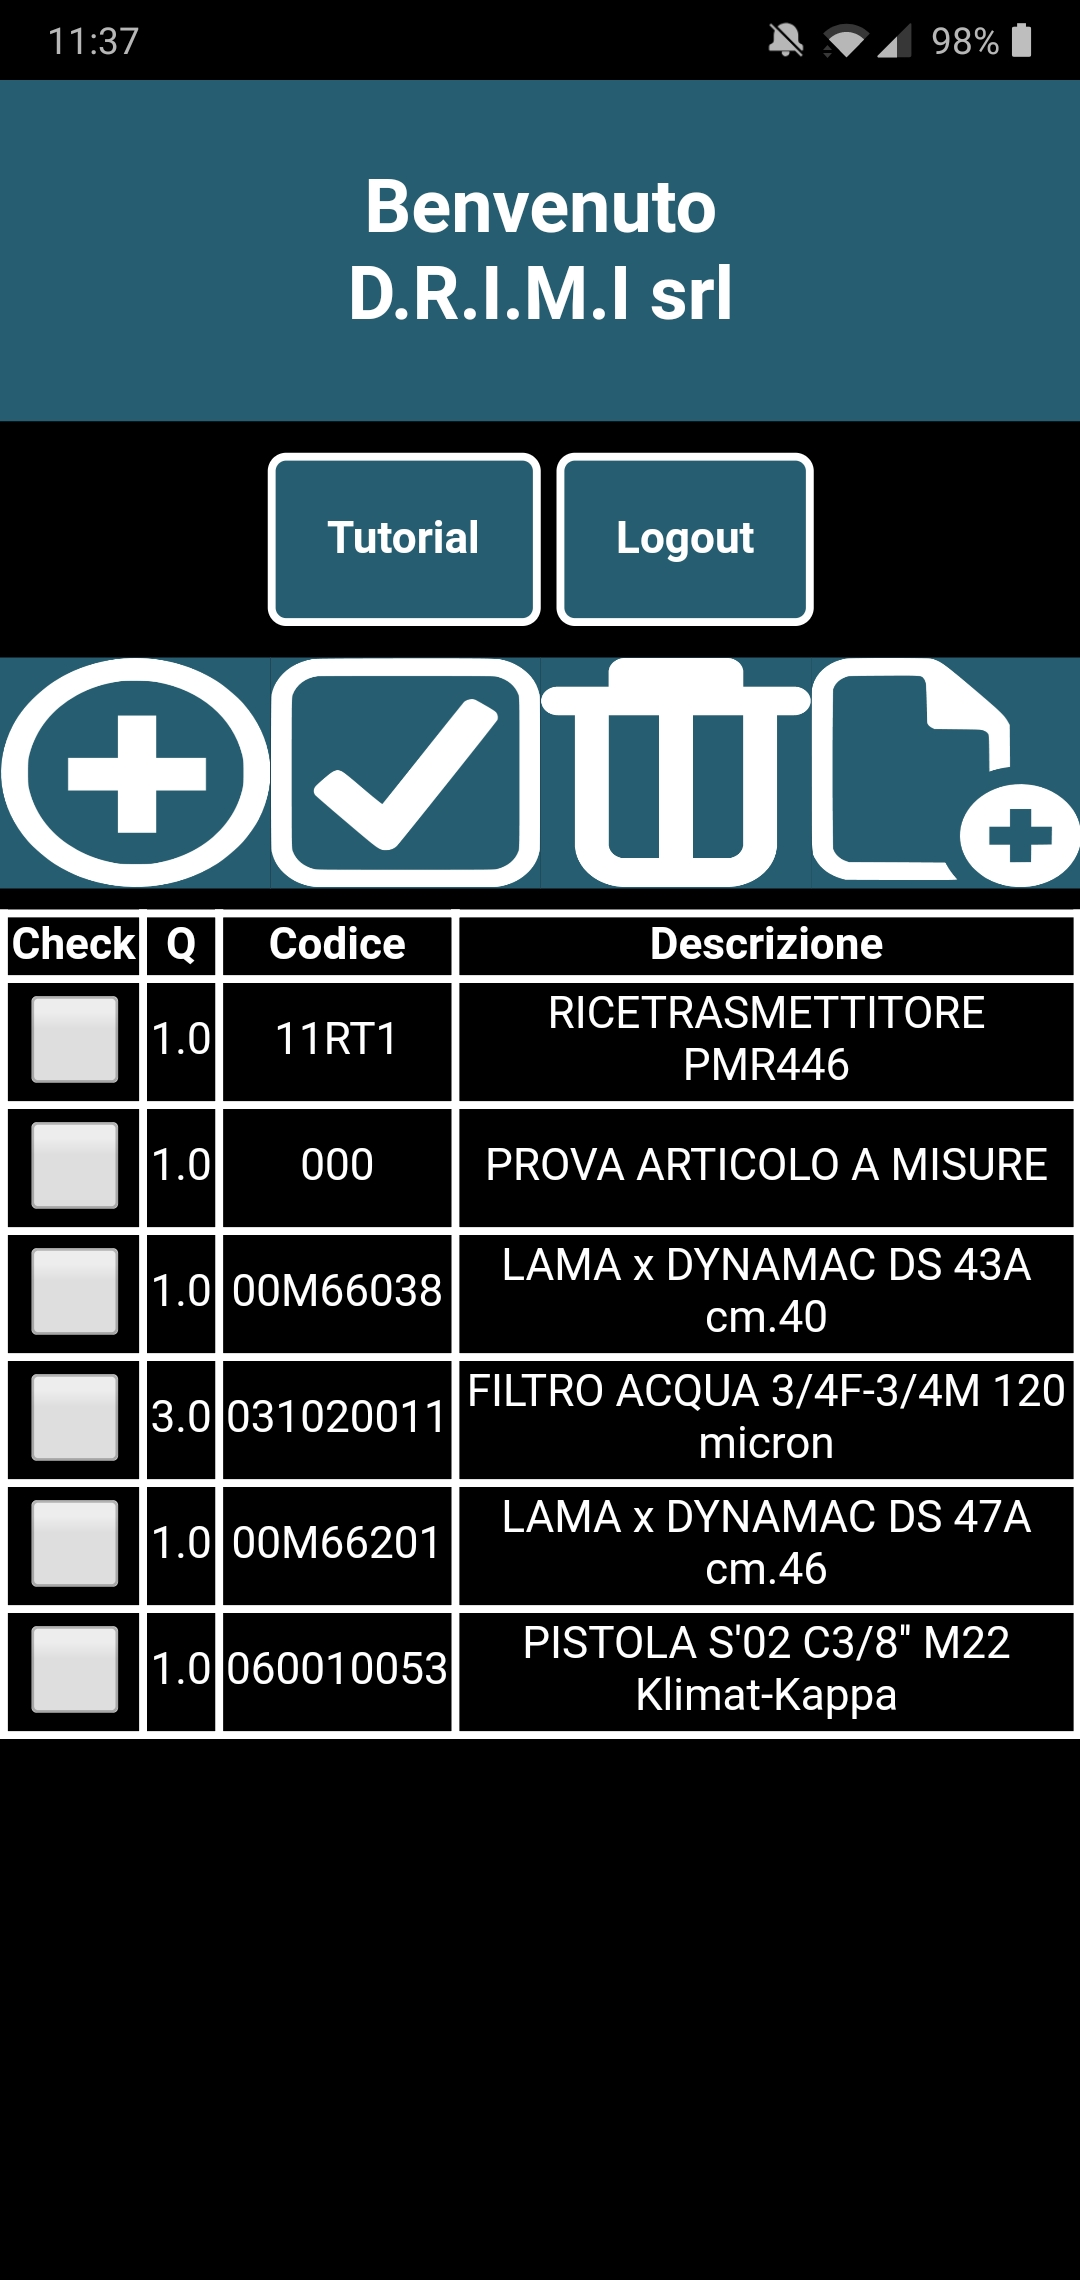
\includegraphics[width=0.4\columnwidth]{interfaccia/home} 
    \caption{Home page}
\end{figure}

La home page racchiude tutte le funzionalità di moviORDER. A partire dall'alto e proseguendo verso il basso l'interfaccia presenta le seguenti parti:
\begin{itemize}
	\item messaggio di benvenuto per l'utente autenticato: questo messaggio visualizza la ragione sociale dell'utente;
	\item pulsante tutorial: premendo su questo pulsante è possibile visualizzare il tutorial di moviORDER;
	\item pulsante logout: premendo su questo pulsante è possibile effettuare il logout da moviORDER;
	\item pulsante di aggiunta articolo: premendo su questo pulsante è possibile accedere al modal per l'aggiunta di un articolo in carrello; 
	\item pulsante di selezione/deselezione multipla di articoli: premendo su questo pulsante è possibile selezionare/deselezionare tutti gli articoli in carrello;
	\item pulsante di eliminazione articoli: premendo su questo pulsante è possibile rimuovere gli articoli selezionati dal carrello;
	\item pulsante di invio ordine: premendo su questo pulsante è possibile accedere al modal di invio ordine;
	\item carrello: ogni articolo in carrello presenta:
	\begin{itemize}
		\item una check-box per la selezione/deselezione dell'articolo;
		\item un'indicazione sulla quantità di pezzi ordinati;
		\item il codice dell'articolo;
		\item una breve descrizione dell'articolo.
	\end{itemize}
\end{itemize}

\subsection{Modal di aggiunta articolo}

\begin{figure}[!h] 
    \centering 
    	\subfloat{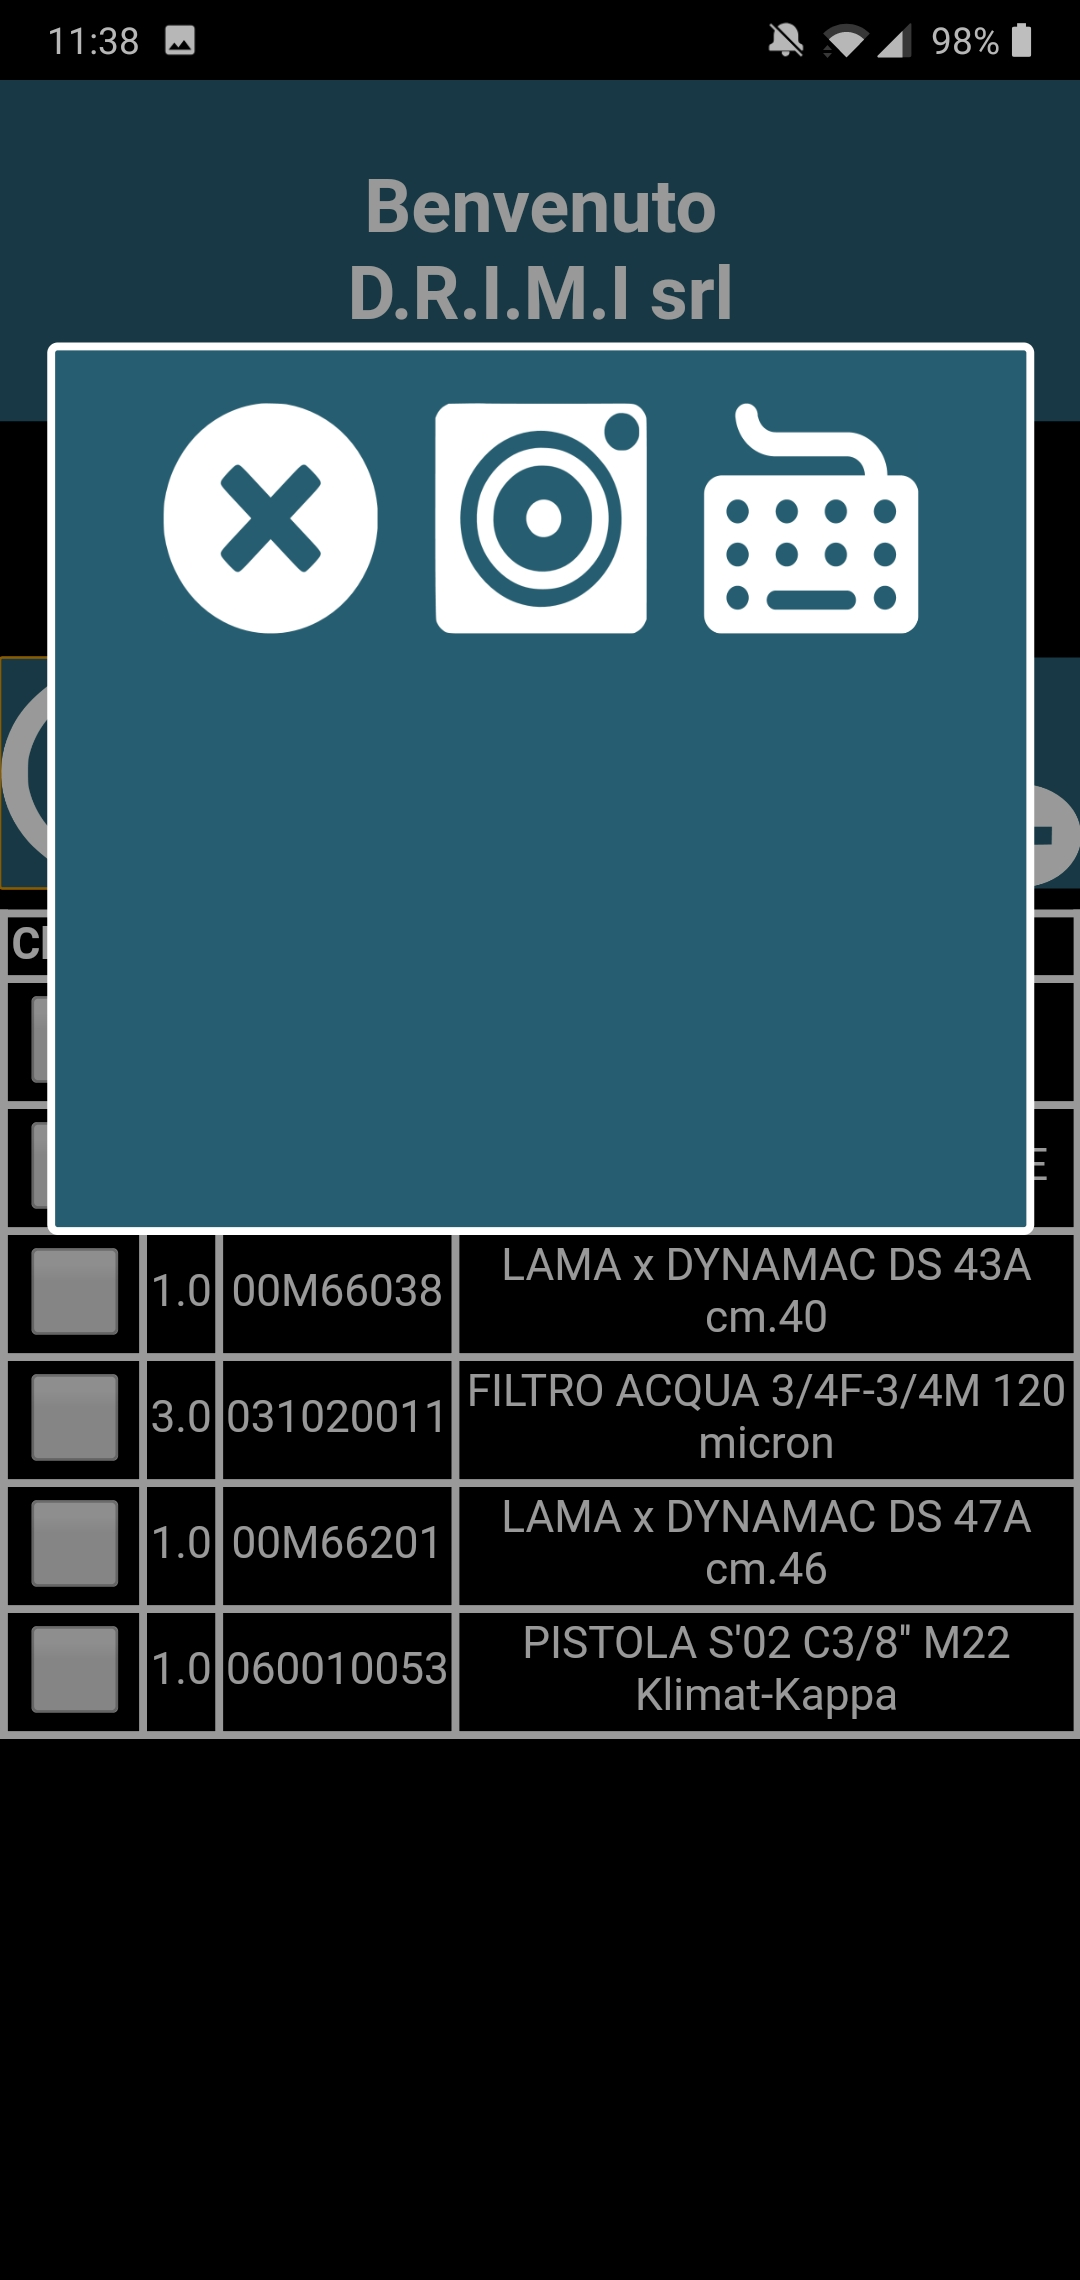
\includegraphics[width=0.33\columnwidth]{interfaccia/modalAggiunta}}
    	\subfloat{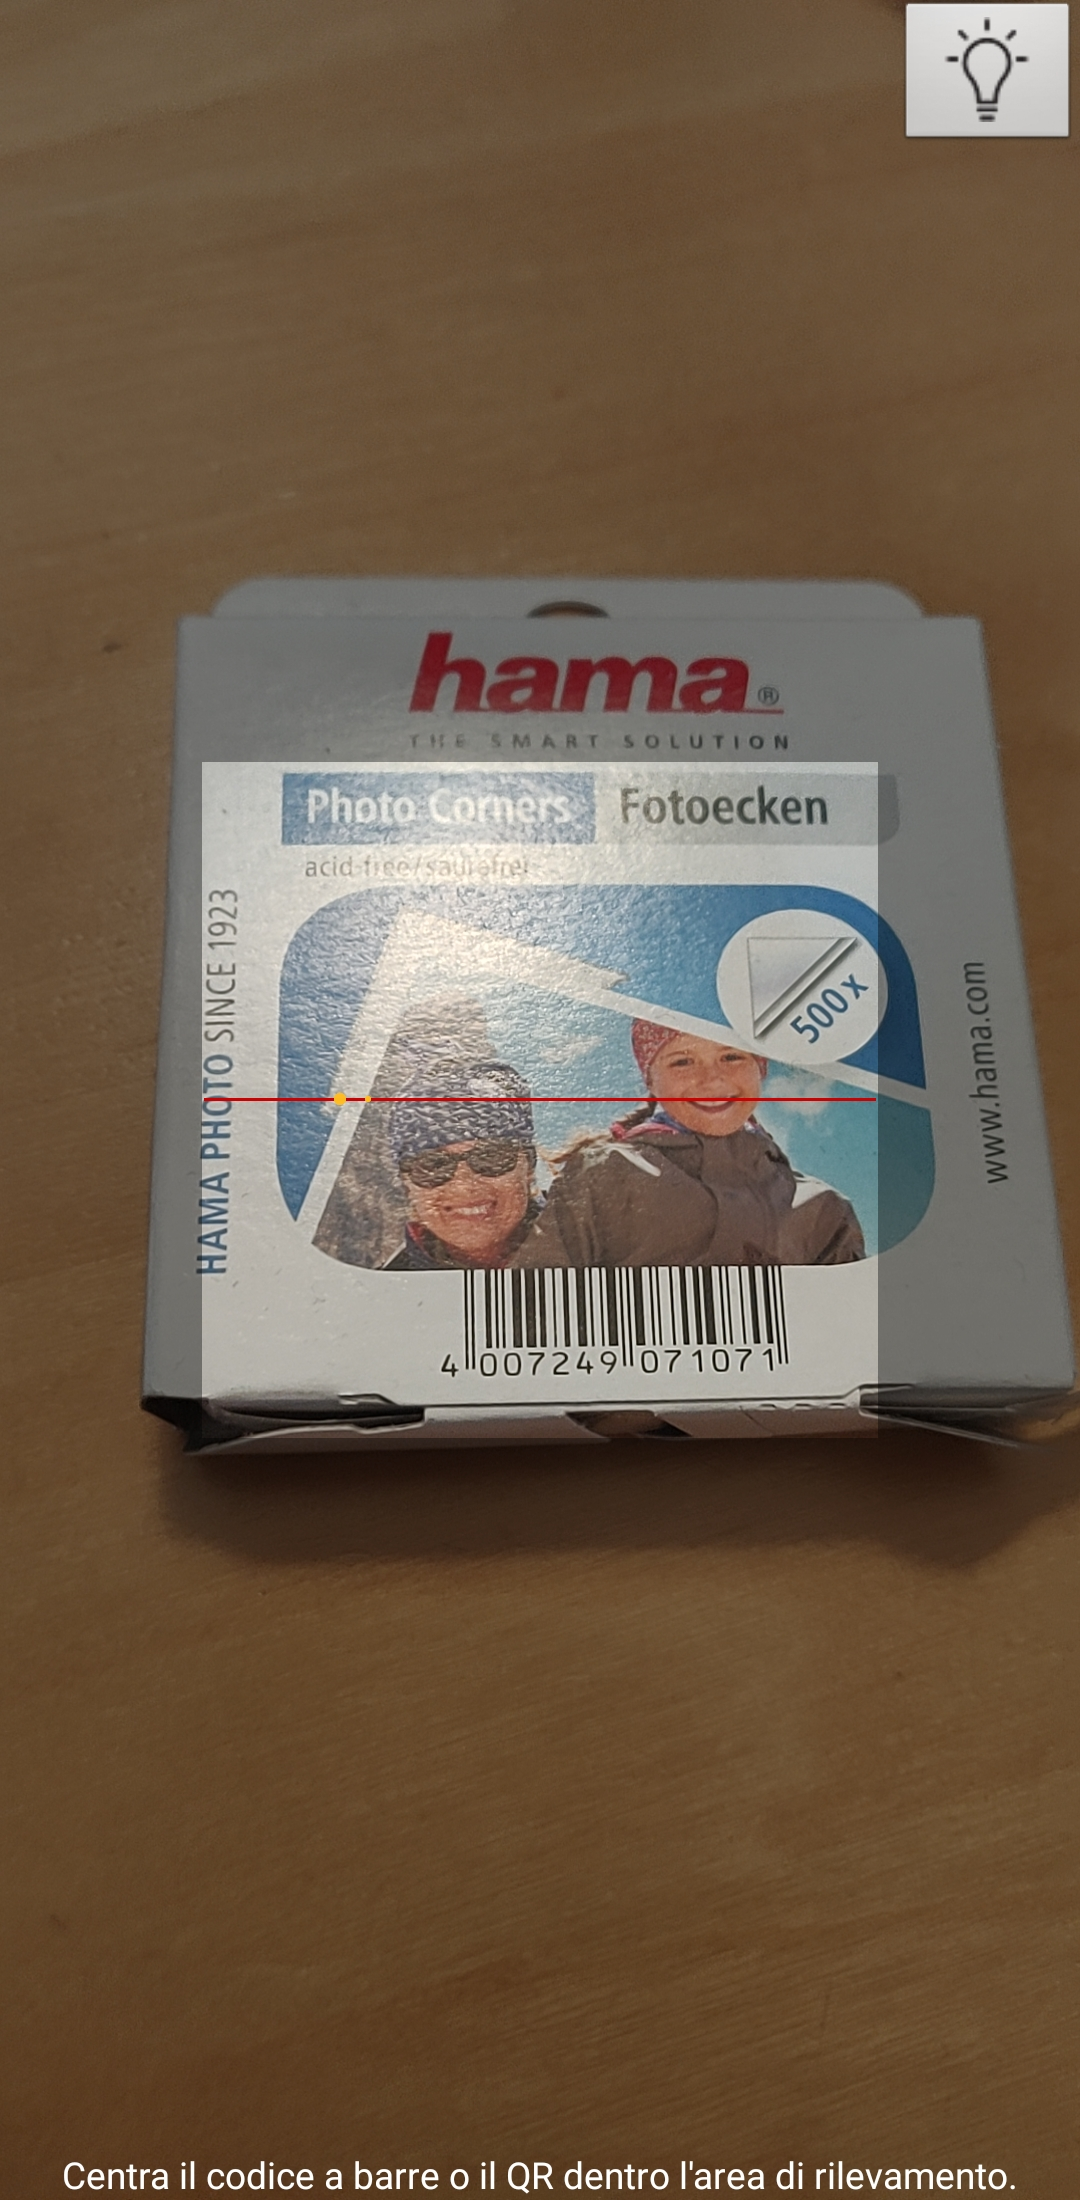
\includegraphics[width=0.33\columnwidth]{interfaccia/scansione}} 
    	\subfloat{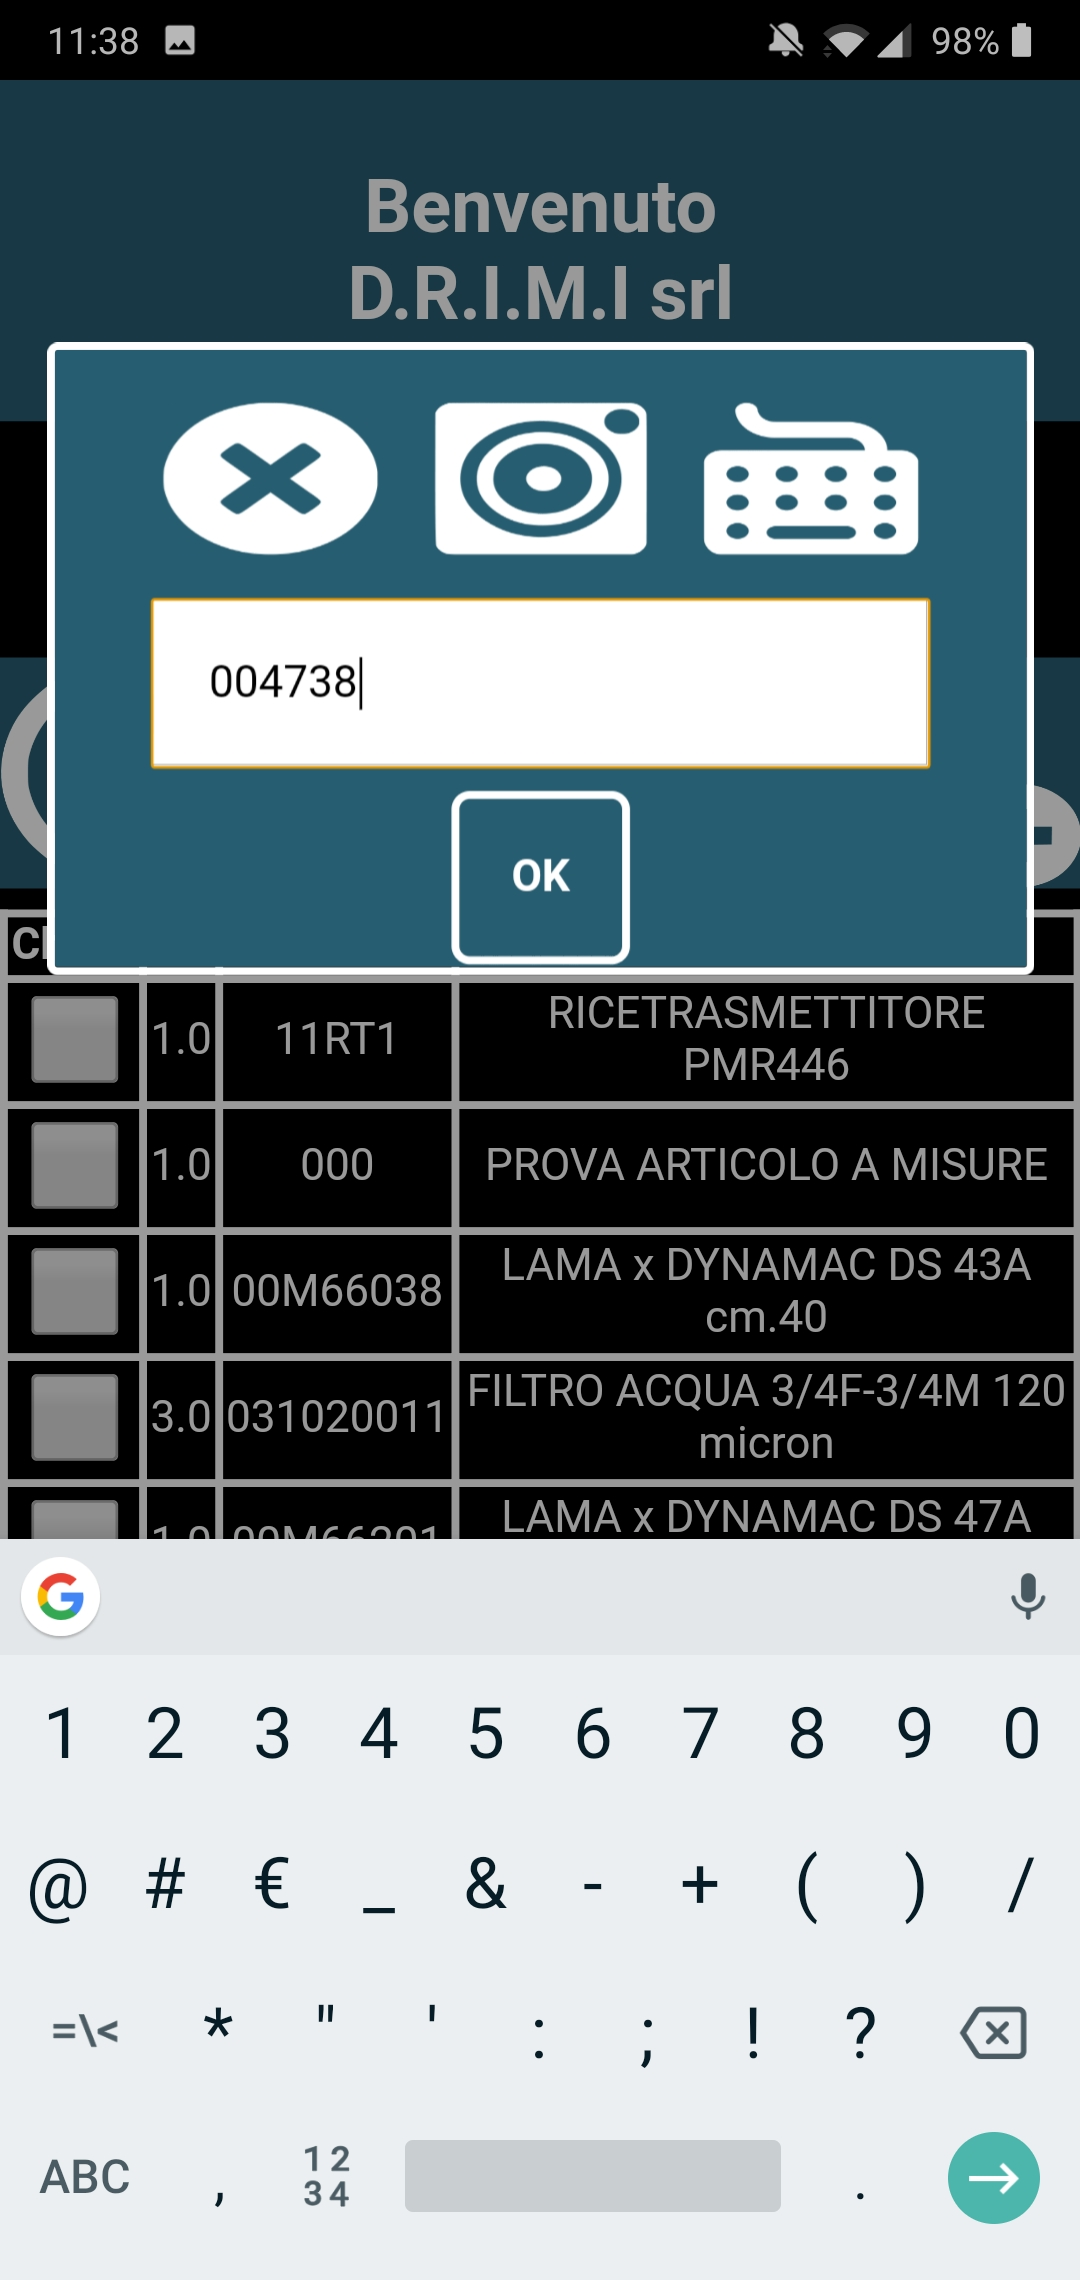
\includegraphics[width=0.33\columnwidth]{interfaccia/manuale}} 
    \caption{Modal di aggiunta articolo e modalità di aggiunta (scansione o inserimento manuale)}
\end{figure}

Il modal di aggiunta articolo permette di decidere la modalità di inserimento dell'articolo in carrello. Il modal presenta di seguenti pulsanti:
\begin{itemize}
	\item annullamento aggiunta: premendo su questo pulsante è possibile tornare alla home page di moviORDER;
	\item scansione codice a barre: premendo su questo pulsante è possibile aggiungere un nuovo articolo scansionando il codice a barre dello stesso. Per la scansione del codice a barre viene aperta la fotocamera del dispositivo;
	\item inserimento manuale: premendo su questo pulsante è possibile aggiungere un nuovo articolo inserendo manualmente il codice dello stesso.
\end{itemize}
Se la scansione del codice a barre o l'inserimento del codice articolo vanno a buon fine, viene aperta la pagina per l'aggiunta dell'articolo corrispondente.

\subsection{Pagina di aggiunta articolo}

\begin{figure}[!h] 
    \centering 
    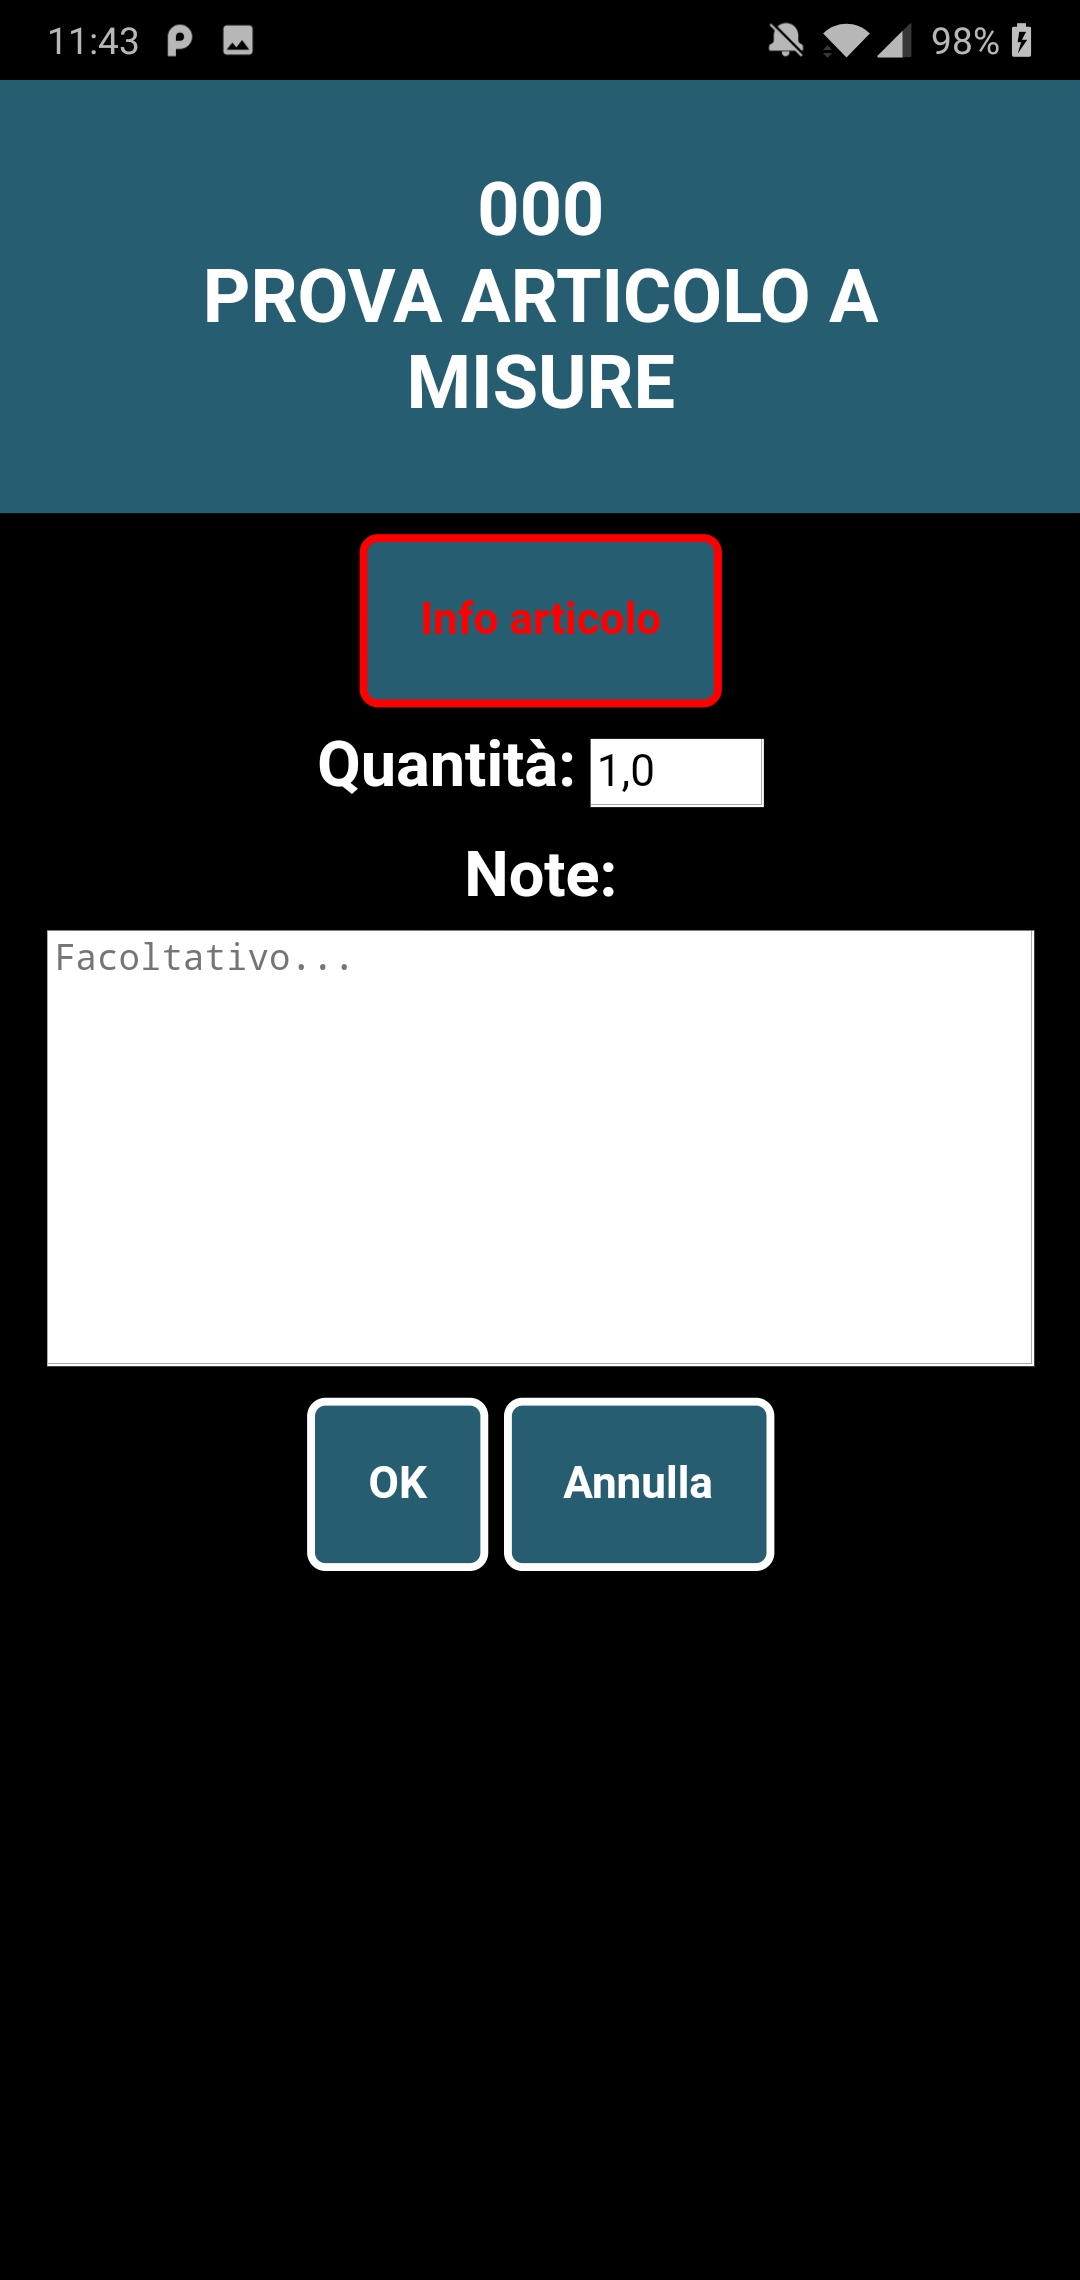
\includegraphics[width=0.4\columnwidth]{interfaccia/aggiunta} 
    \caption{Pagina di aggiunta articolo}
\end{figure}

La pagina di aggiunta articolo permette di aggiungere un nuovo articolo al carrello e presenta le seguenti parti:
\begin{itemize}
	\item codice e nome articolo: in base al codice precedentemente scansionato o inserito, vengono visualizzate le informazioni relative al codice articolo e al nome dell'articolo;
	\item pulsante di visualizzazione informazioni dell'articolo: premendo questo pulsante è possibile visualizzare le informazioni dell'articolo che si sta aggiungendo al carrello. Se il pulsante presenta bordo rosso significa che per l'articolo non sono presenti informazioni. Questo permette all'utente di evitare un tap inutile;
	\item text-box per l'inserimento della quantità: tramite questa text-box è possibile inserire la quantità da ordinare per l'articolo che si sta aggiungendo al carrello;
	\item text-area per l'inserimento delle note: tramite questa text-area è possibile inserire delle note facoltative per l'articolo che si sta aggiungendo al carrello;
	\item pulsante di conferma: tramite questo pulsante è possibile confermare l'aggiunta dell'articolo in carrello;
	\item pulsante di annullamento: tramite questo pulsante è possibile annullare l'aggiunta dell'articolo in carrello e tornare alla home page di moviORDER.
\end{itemize}

\subsection{Pagina di modifica articolo}

Dalla home page di moviORDER premendo su un qualsiasi articolo in carrello è possibile modificare i dati d'ordine di tale articolo. Alla pressione dell'articolo viene aperta la pagina di modifica articolo. Questa pagina è identica alla pagina di aggiunta articolo ma contiene i dati precedentemente inseriti per l'articolo. È possibile modificare i dati precedentemente inseriti eseguendo le stesse interazioni previste per la pagina di aggiunta articolo.

\subsection{Modal di invio ordine}

\begin{figure}[!h] 
    \centering 
    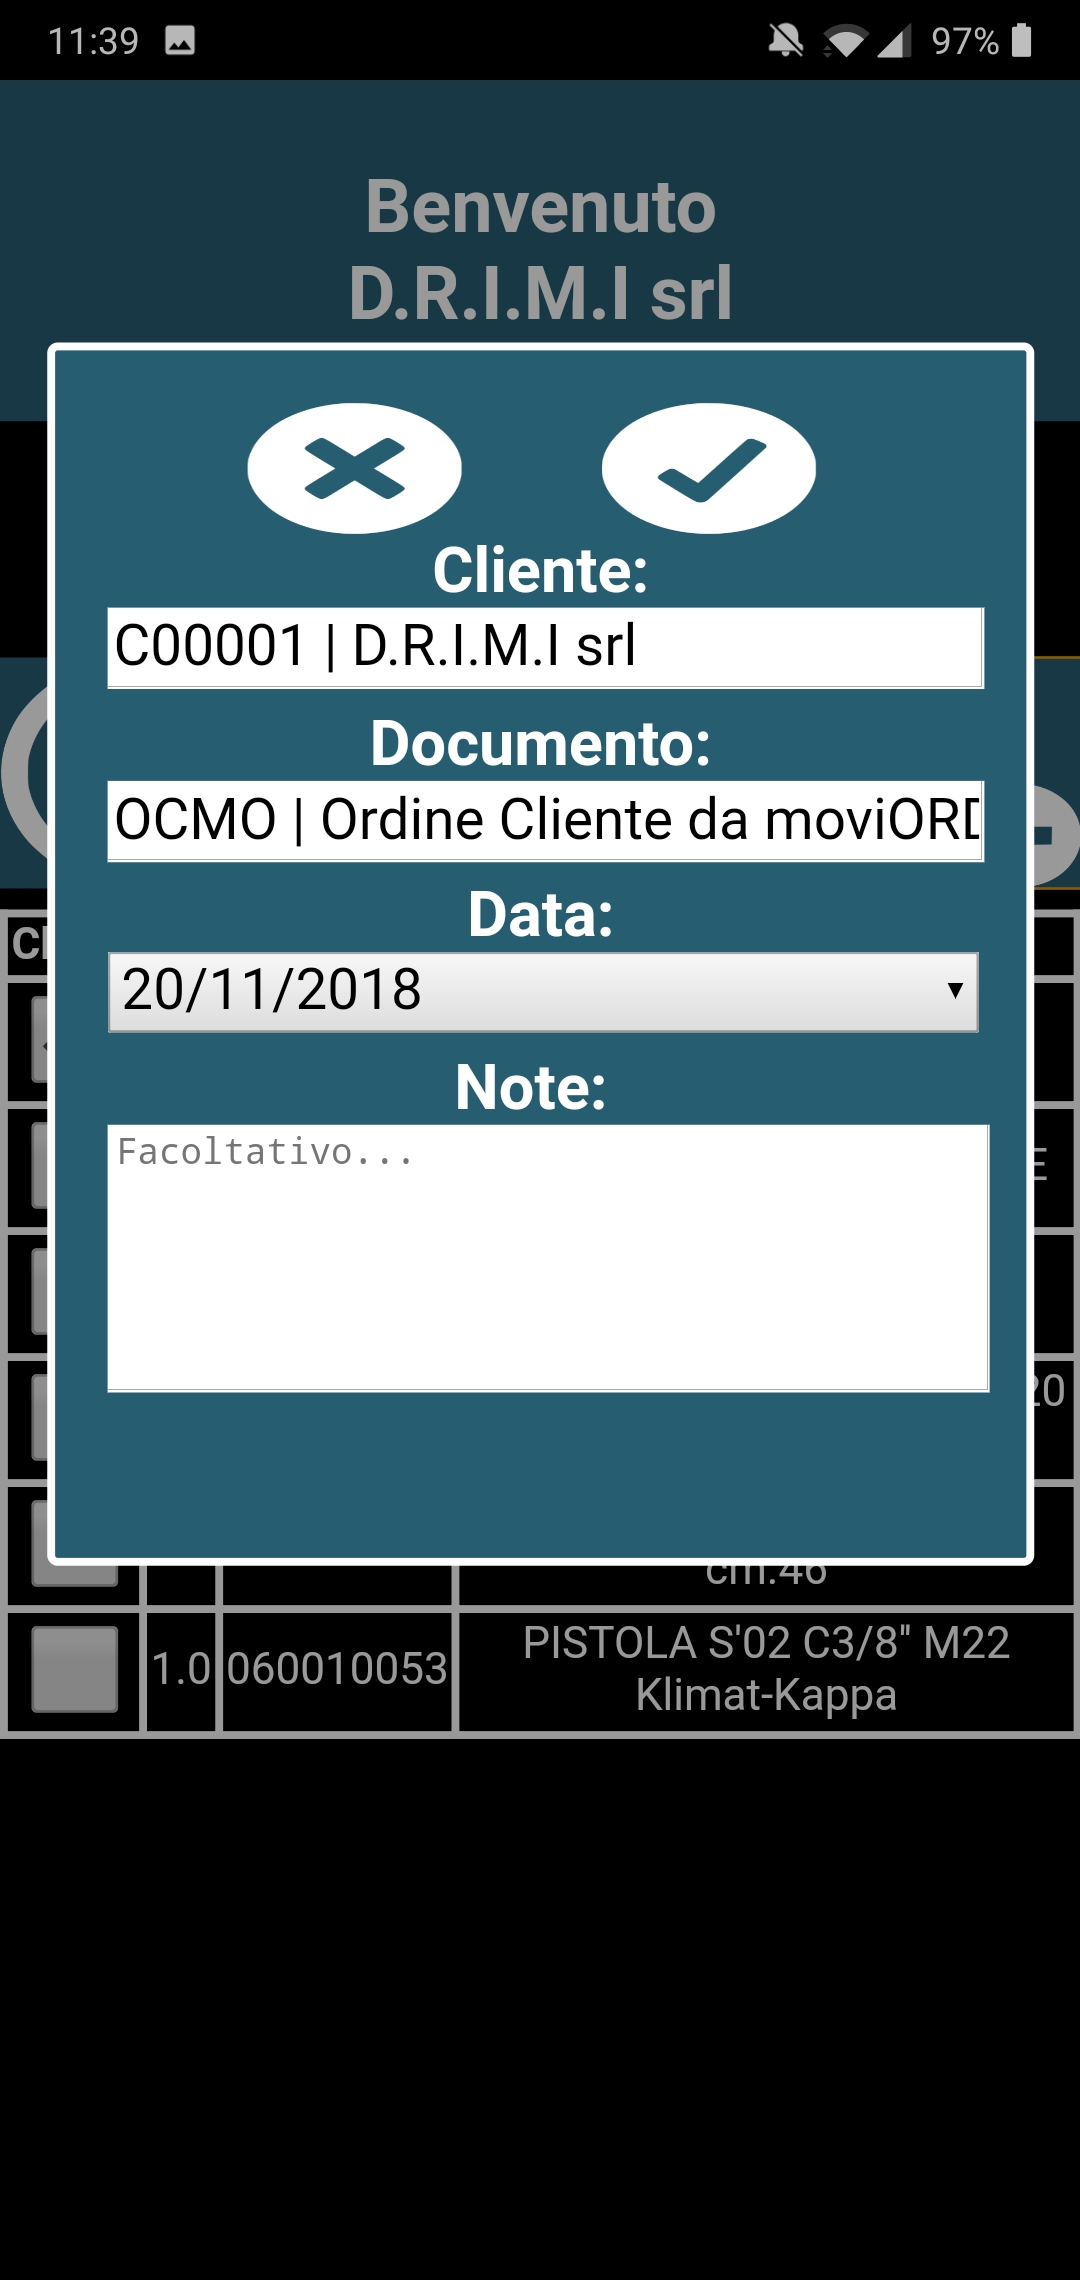
\includegraphics[width=0.4\columnwidth]{interfaccia/modalInvio} 
    \caption{Modal di invio ordine}
\end{figure}

Il modal di invio ordine permette di inviare un ordine alla propria azienda. Tale ordine contiene tutti gli articoli precedentemente selezionati dal carrello. Il modal presenta le seguenti parti:
\begin{itemize}
	\item pulsante di annullamento: premendo questo pulsante è possibile annullare l'invio dell'ordine e tornare alla home page di moviORDER;
	\item pulsante di conferma: tramite questo pulsante è possibile confermare l'invio dell'ordine;
	\item informazioni sul cliente: questa text-box contiene il codice e la ragione sociale del cliente che sta effettuando l'ordine;
	\item informazioni sul documento: questa text-box contiene il codice e la descrizione del documento che deve essere generato una volta inviato l'ordine;
	\item select per l'inserimento della data: questa select permette l'inserimento della data d'ordine. Di default viene proposta la data corrente;
	\item text-area per l'inserimento delle note: questa text-area permette di inserire delle note facoltative per l'ordine che si sta inviando.
\end{itemize}


\textbf{per la parte di progettazione far vedere che il database potrebbe essere anche sul server di un'azienda esterna, commonDB sempre sul server vision mentre il db dell'azienda può essere su un server esterno.}
